\section[Data to Monte Carlo comparisons at $\sqrt{s}=2.36$ TeV in
  Minimum Bias events]{Data to Monte Carlo comparisons at $\boldsymbol{\sqrt{s}=2.36}$ TeV in
  Minimum Bias events}
\label{sc:DataVsMCMB2360}

In this section we present the comparison of several calorimeter-based $\etmiss$ and $\sumet$
distributions between data and {\sc pythia} Minimum Bias Monte Carlo simulation at $\sqrt{s}=2360$~GeV. 
All distributions shown in this section are required to pass the trigger and event selections
described before (including the noise cleaning for ECAL spikes and HF PMT hits). 
The Monte Carlo distributions shown in this section
are normalized so that the total number of events in Monte Carlo sample
mathces the number of events observed in data.

\subsection[Basic $\etmiss$-related distributions]{Basic $\etmissB$-related distributions}
\begin{figure}[h!]
 \centering
 \begin{tabular}{ll}
  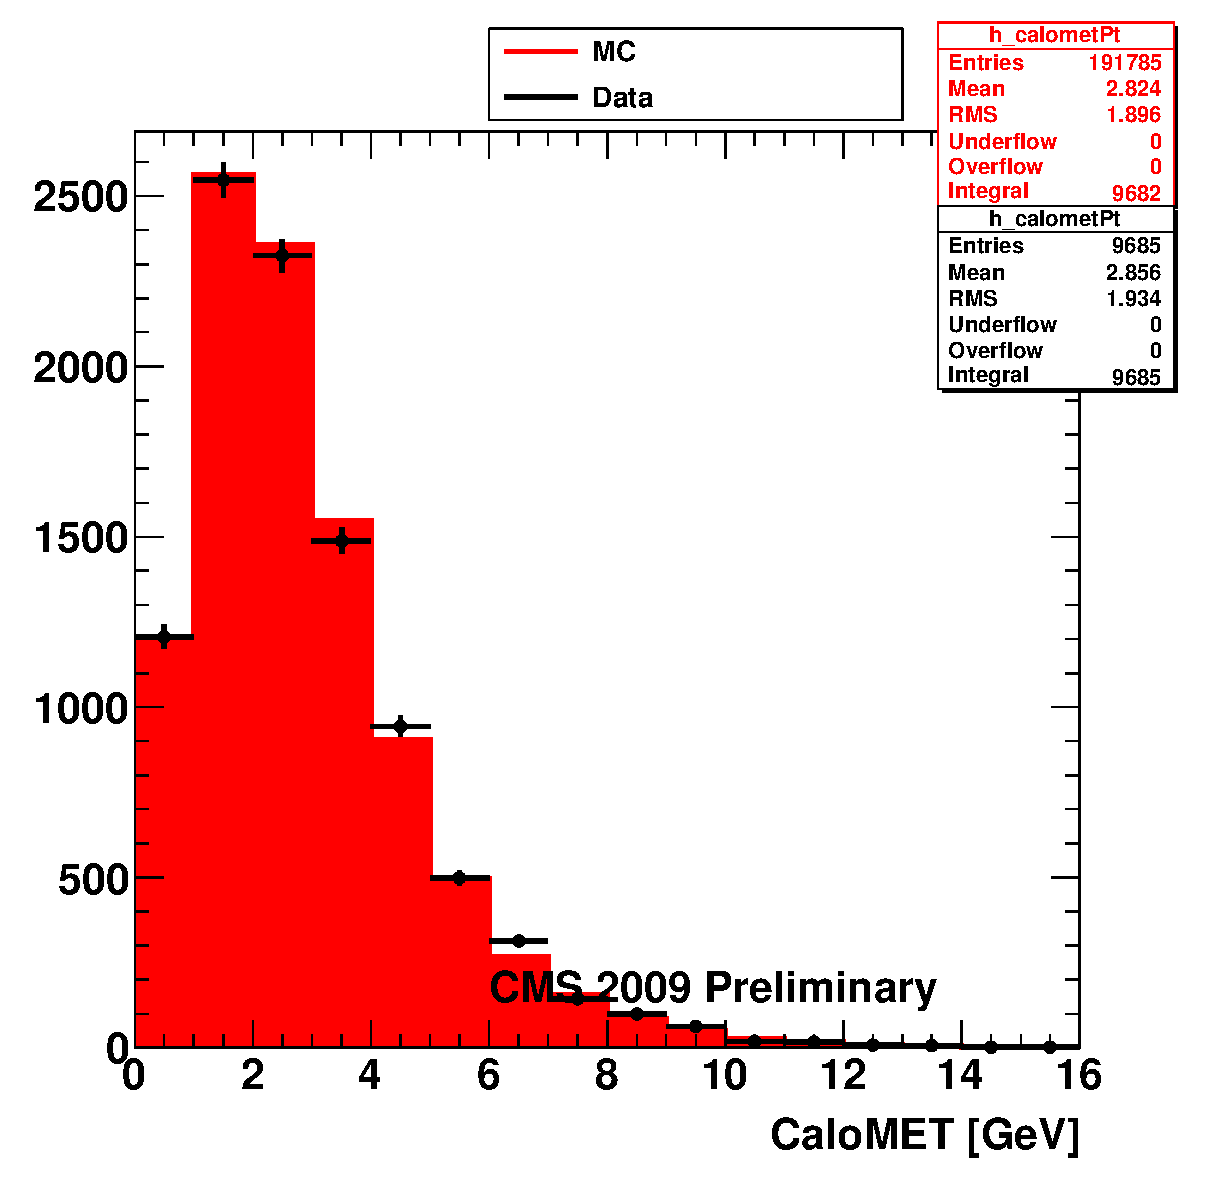
\includegraphics[width=0.40\textwidth]{plots_DataVsMC_MB_2360GeV/h_calometPt_lin.eps} &
  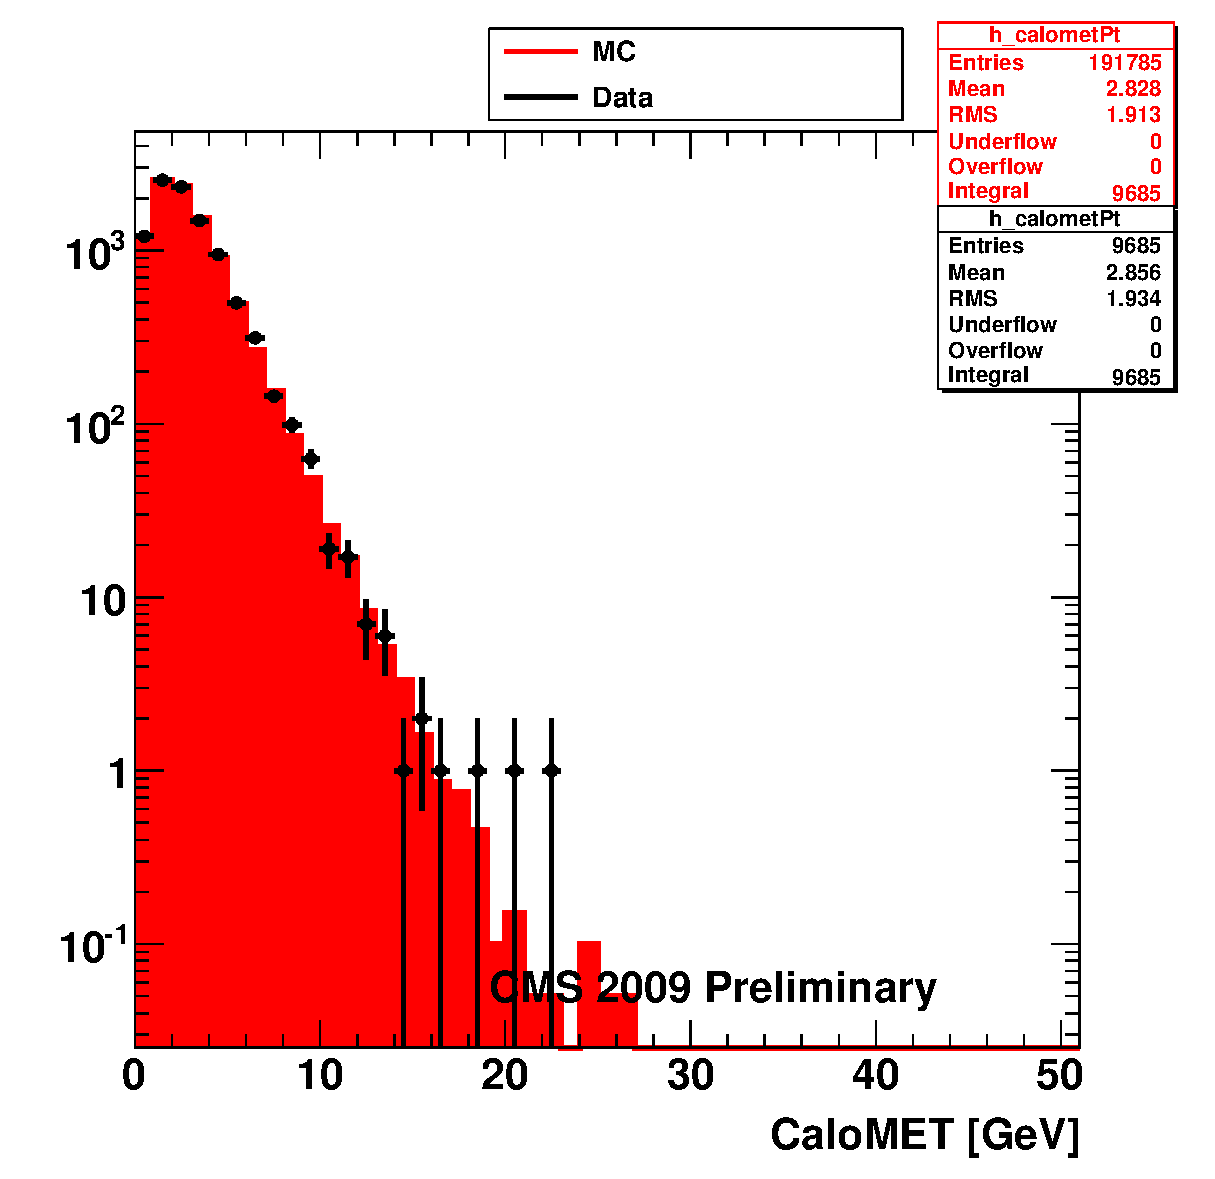
\includegraphics[width=0.40\textwidth]{plots_DataVsMC_MB_2360GeV/h_calometPt.eps} \\
 \end{tabular}
 \caption{$\etmiss$ distributions in 900 GeV data compared
   with Monte Carlo simulation. Same distribution is shown in linear (left) and log (right) scales
   \label{fig:DataVsMC_MB_2360_1}}
\end{figure}

\begin{figure}[h!]
 \centering
 \begin{tabular}{ll}
  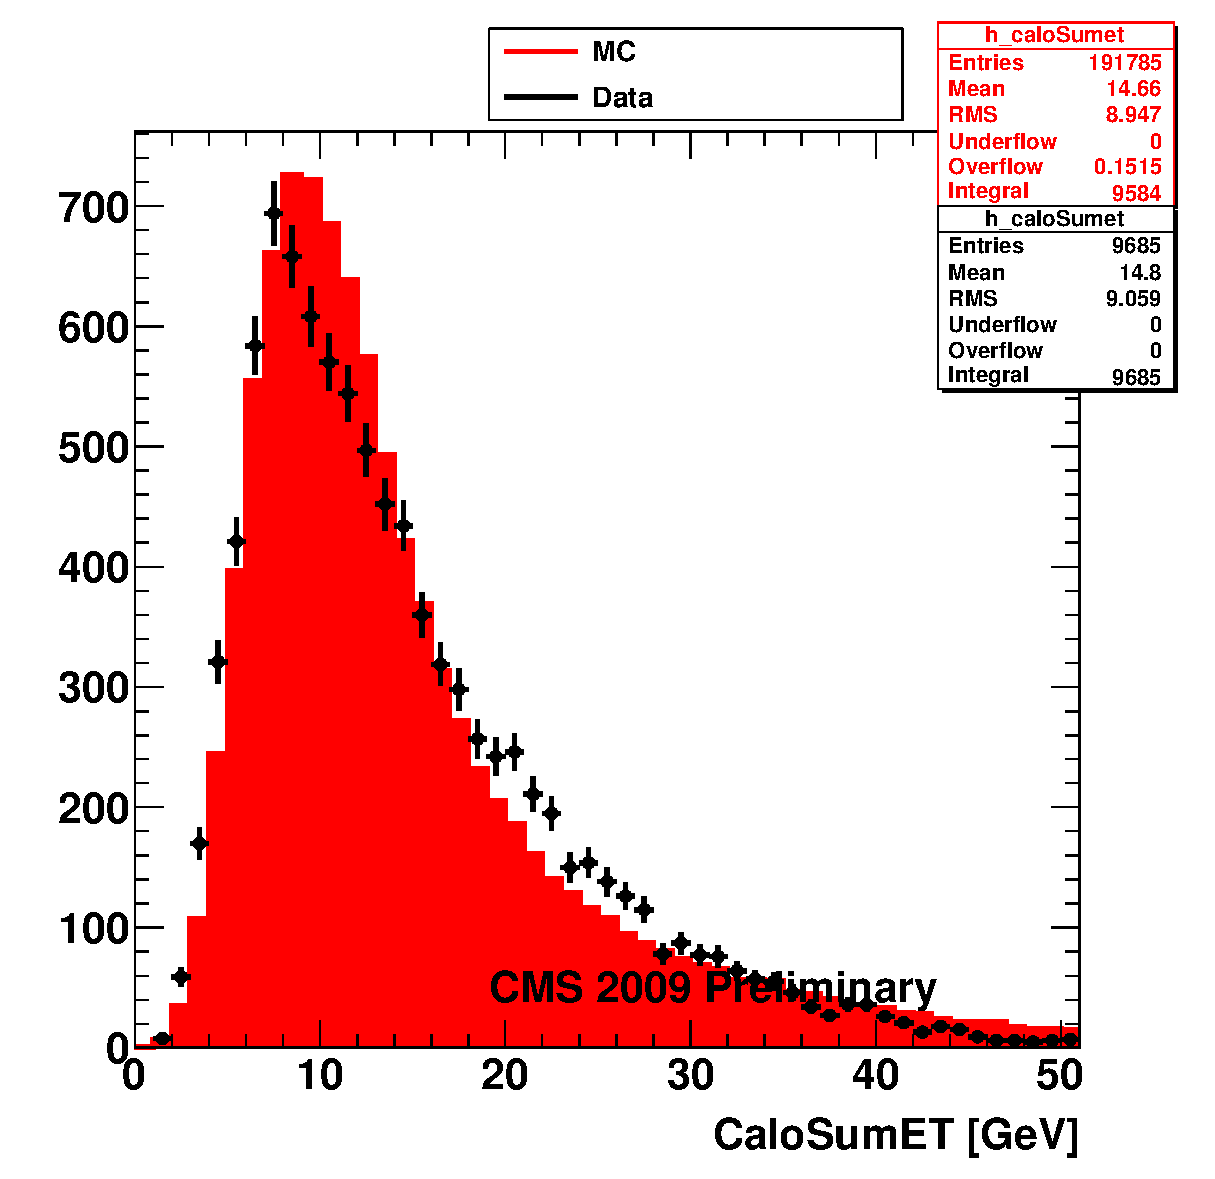
\includegraphics[width=0.40\textwidth]{plots_DataVsMC_MB_2360GeV/h_caloSumet_lin.eps} &
  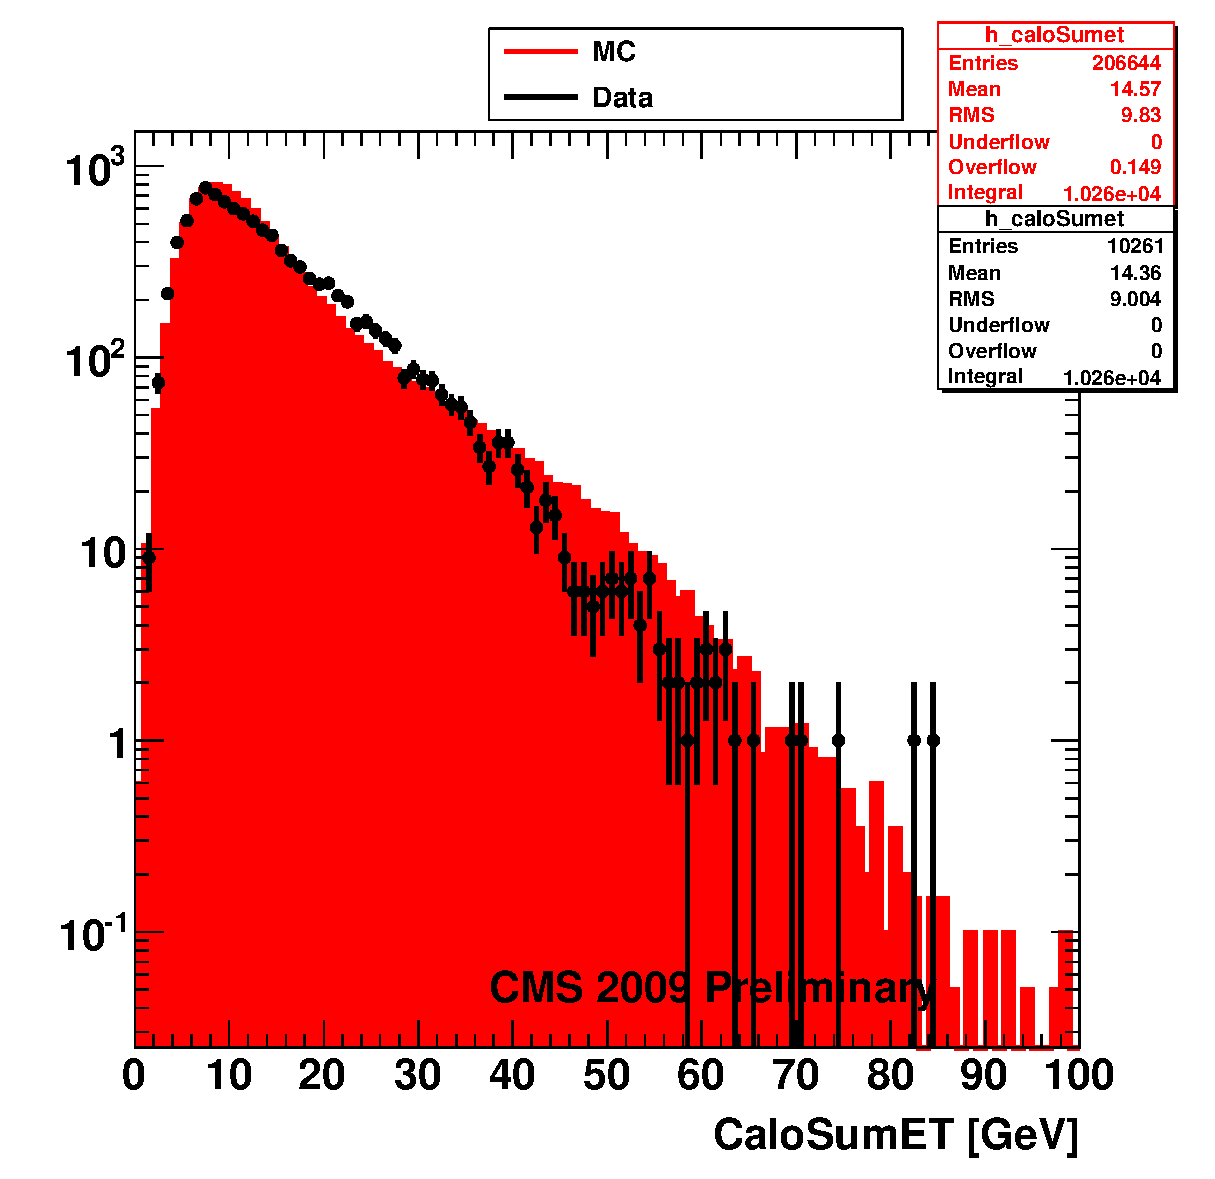
\includegraphics[width=0.40\textwidth]{plots_DataVsMC_MB_2360GeV/h_caloSumet.eps} \\
 \end{tabular}
 \caption{SumET distributions in 2360 GeV data compared
   with Monte Carlo simulation. Same distribution is shown in linear (left) and log (right) scales
          \label{fig:DataVsMC_MB_2360_2}}
\end{figure}

\begin{figure}[h!]
 \centering
 \begin{tabular}{ll}
  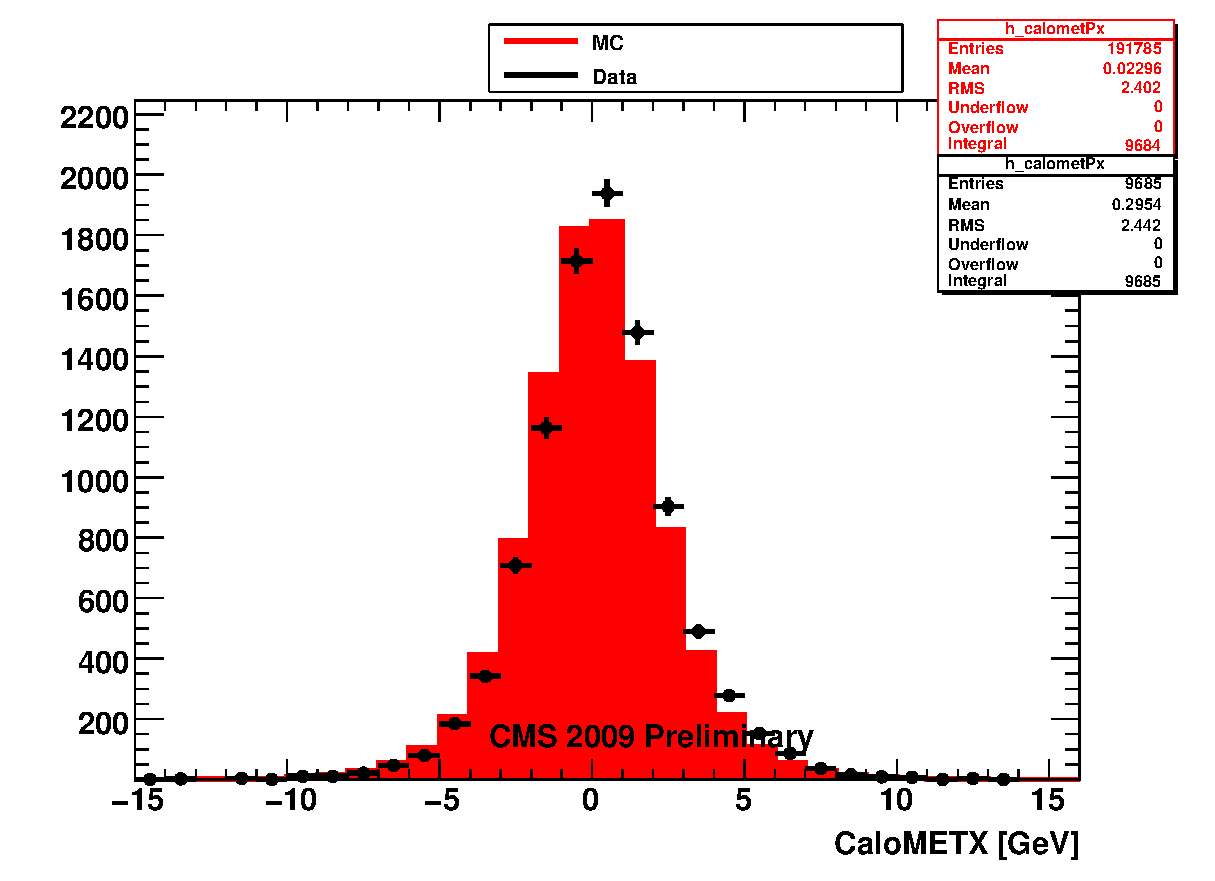
\includegraphics[width=0.40\textwidth]{plots_DataVsMC_MB_2360GeV/h_calometPx_lin.eps} &
  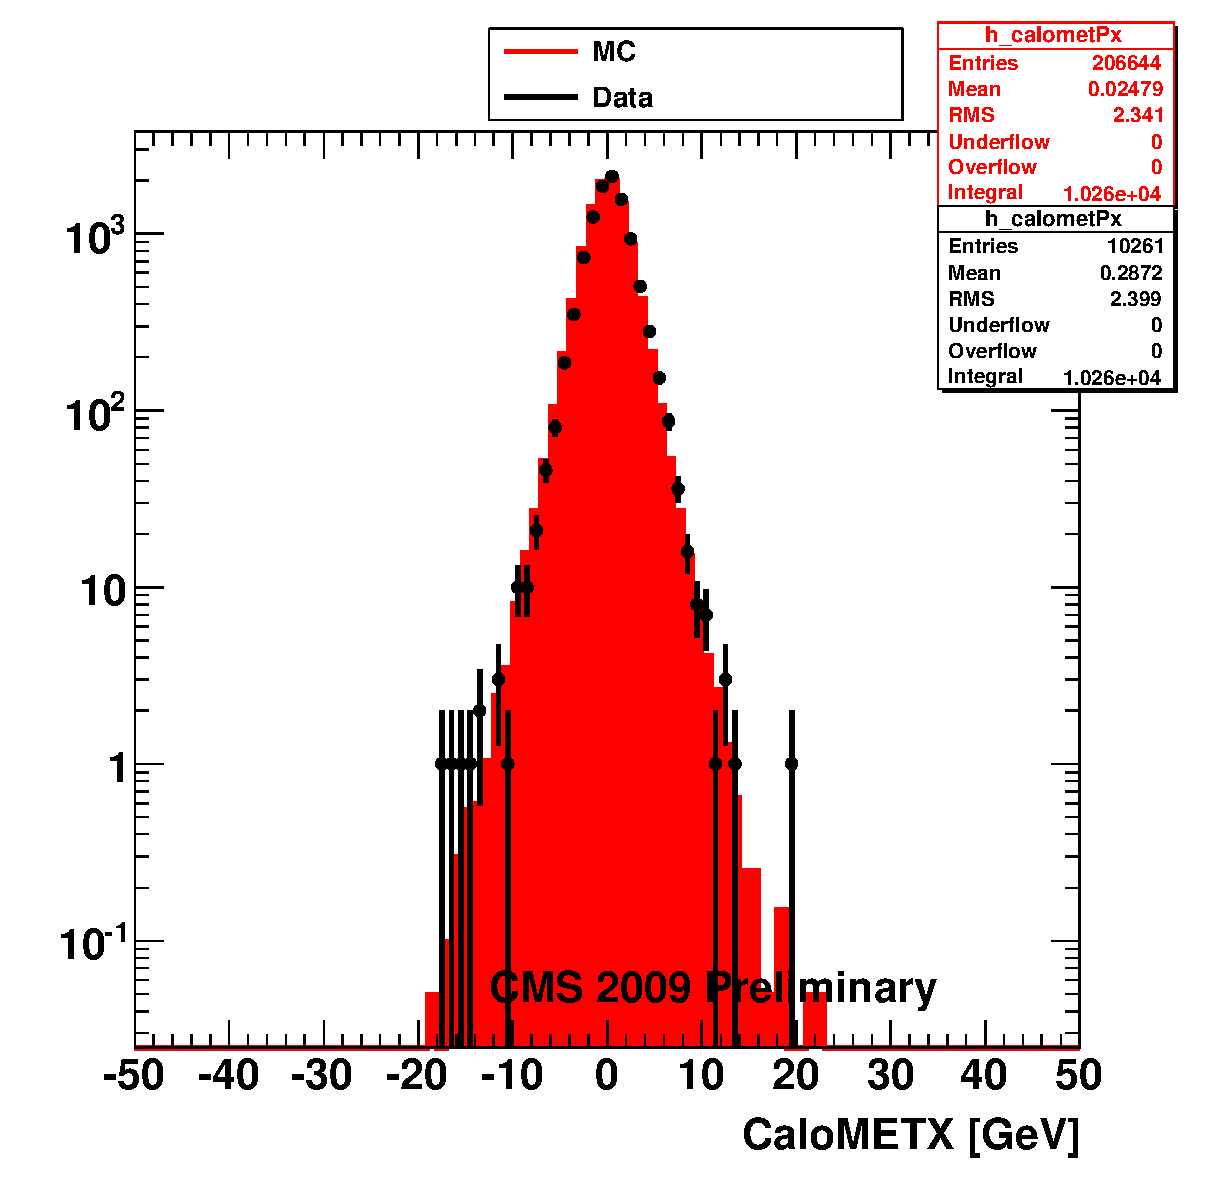
\includegraphics[width=0.40\textwidth]{plots_DataVsMC_MB_2360GeV/h_calometPx.eps} \\
 \end{tabular}
 \caption{$\exmiss$ distributions in 2360 GeV data compared
   with Monte Carlo simulation. Same distribution is shown in linear (left) and log (right) scales
          \label{fig:DataVsMC_MB_2360_3}}
\end{figure}

\begin{figure}[h!]
 \centering
 \begin{tabular}{ll}
  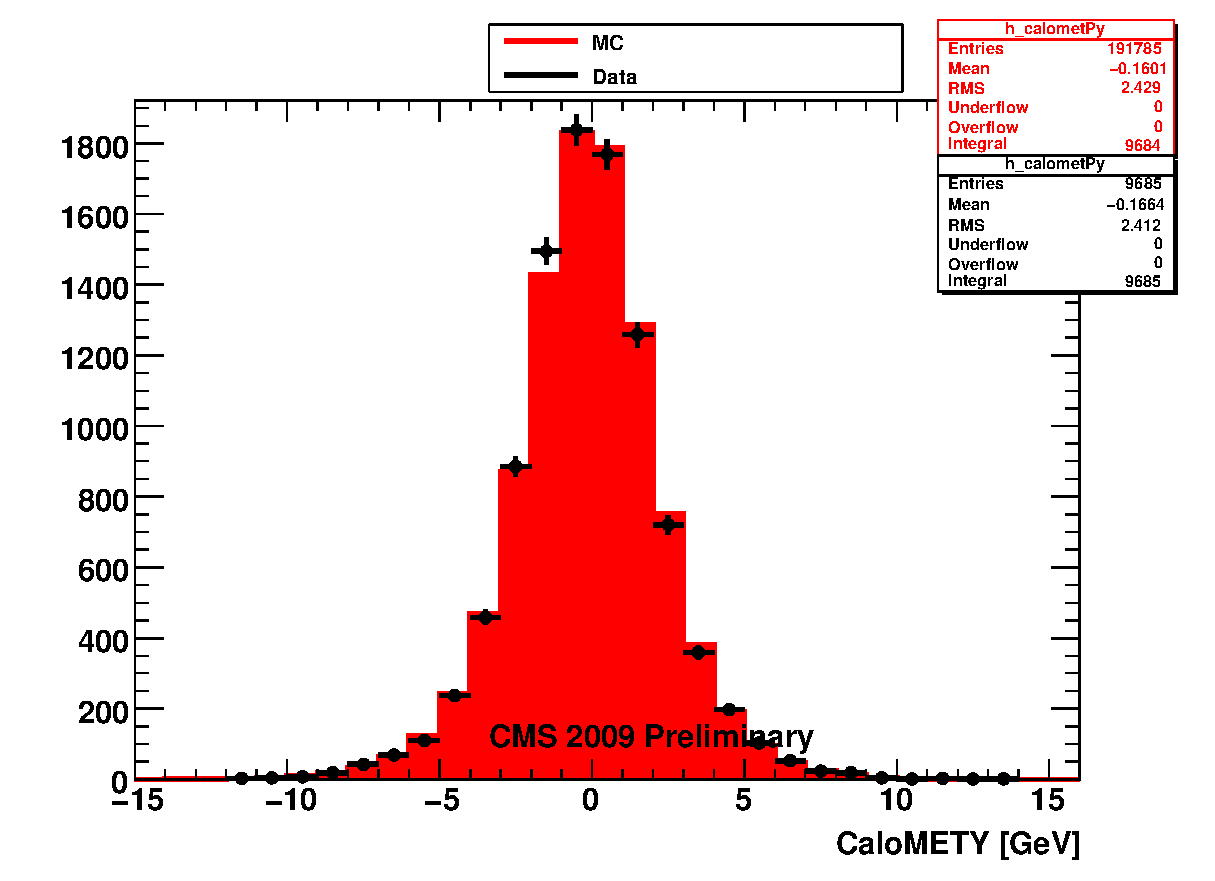
\includegraphics[width=0.40\textwidth]{plots_DataVsMC_MB_2360GeV/h_calometPy_lin.eps} &
  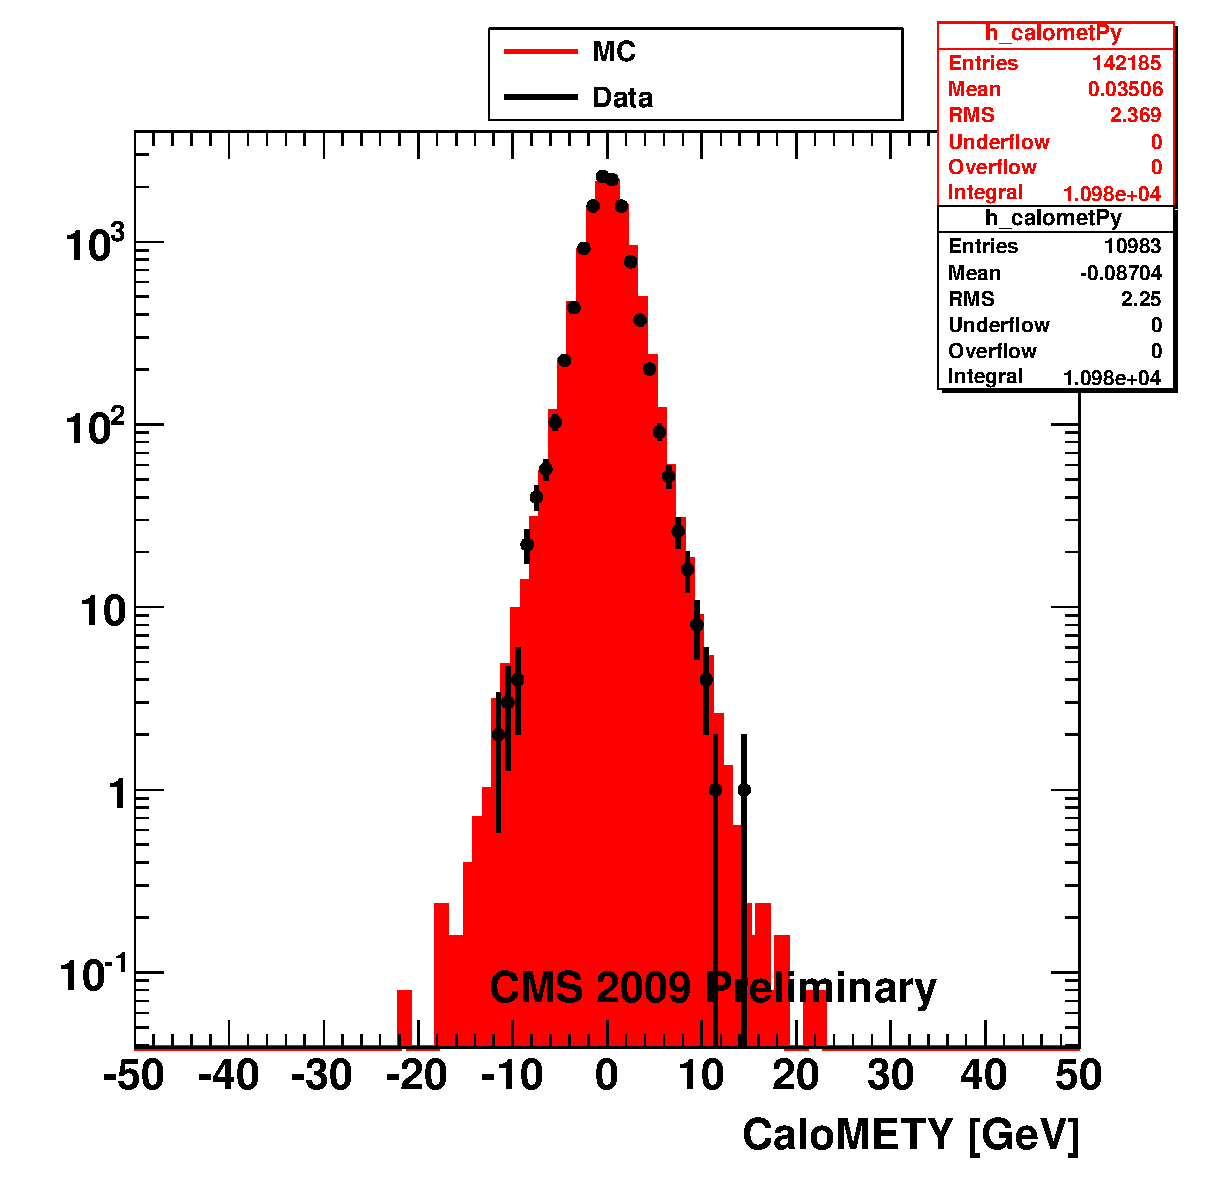
\includegraphics[width=0.40\textwidth]{plots_DataVsMC_MB_2360GeV/h_calometPy.eps} \\
 \end{tabular}
 \caption{$\eymiss$ distributions in 2360 GeV data compared
   with Monte Carlo simulation. Same distribution is shown in linear (left) and log (right) scales
   \label{fig:DataVsMC_MB_2360_4}}
\end{figure}

\begin{figure}[h!]
 \centering
 \begin{tabular}{ll}
  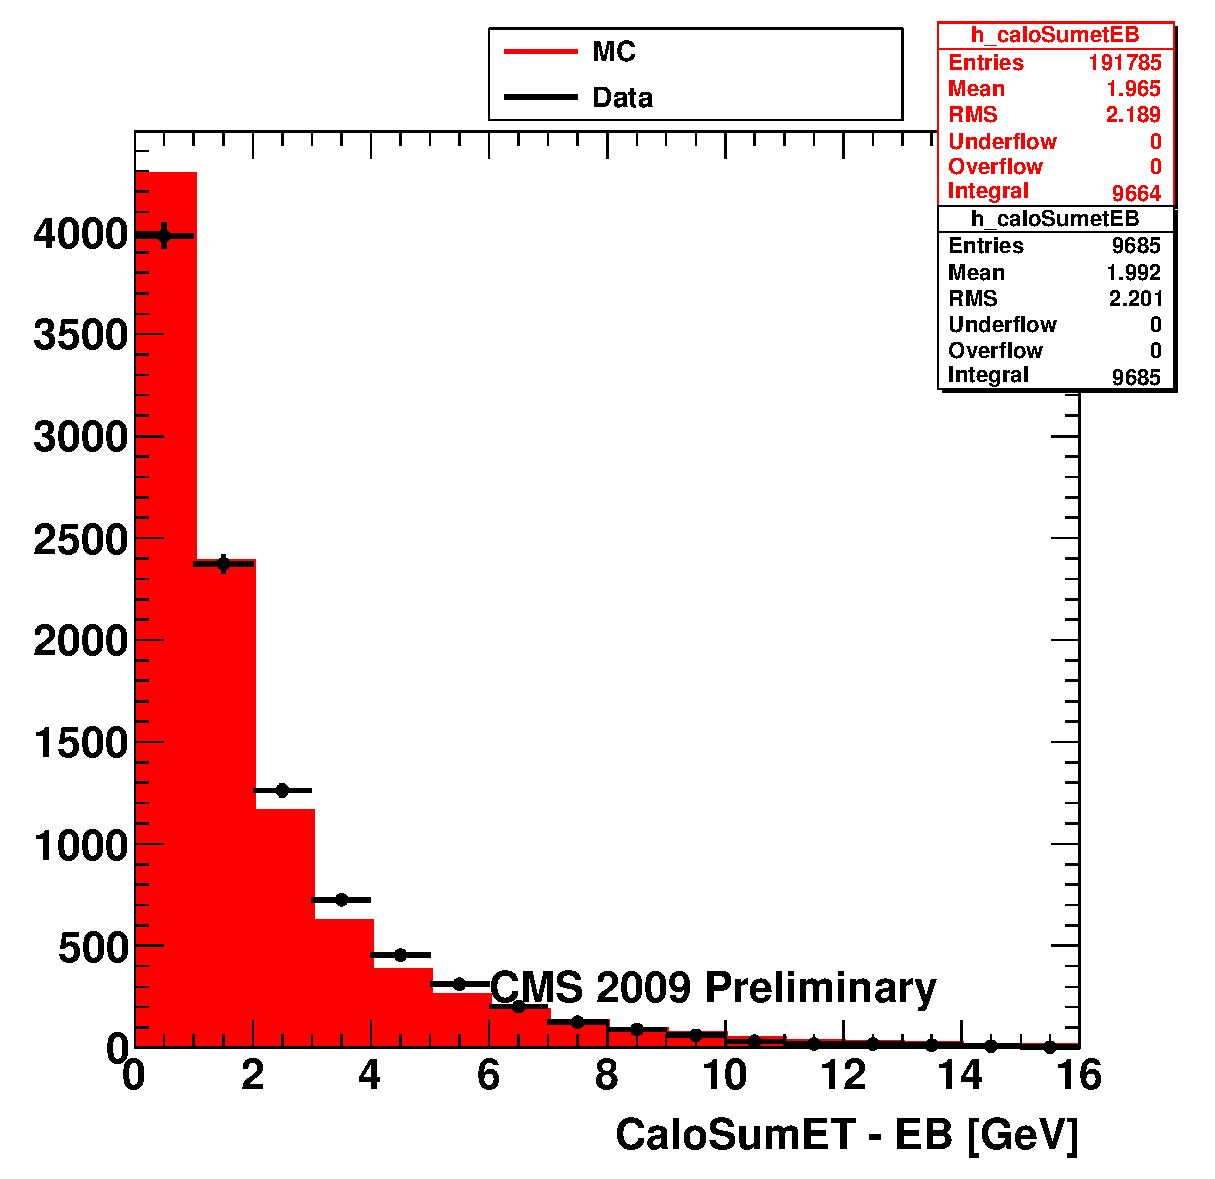
\includegraphics[width=0.40\textwidth]{plots_DataVsMC_MB_2360GeV/h_caloSumetEB_lin.eps} &
  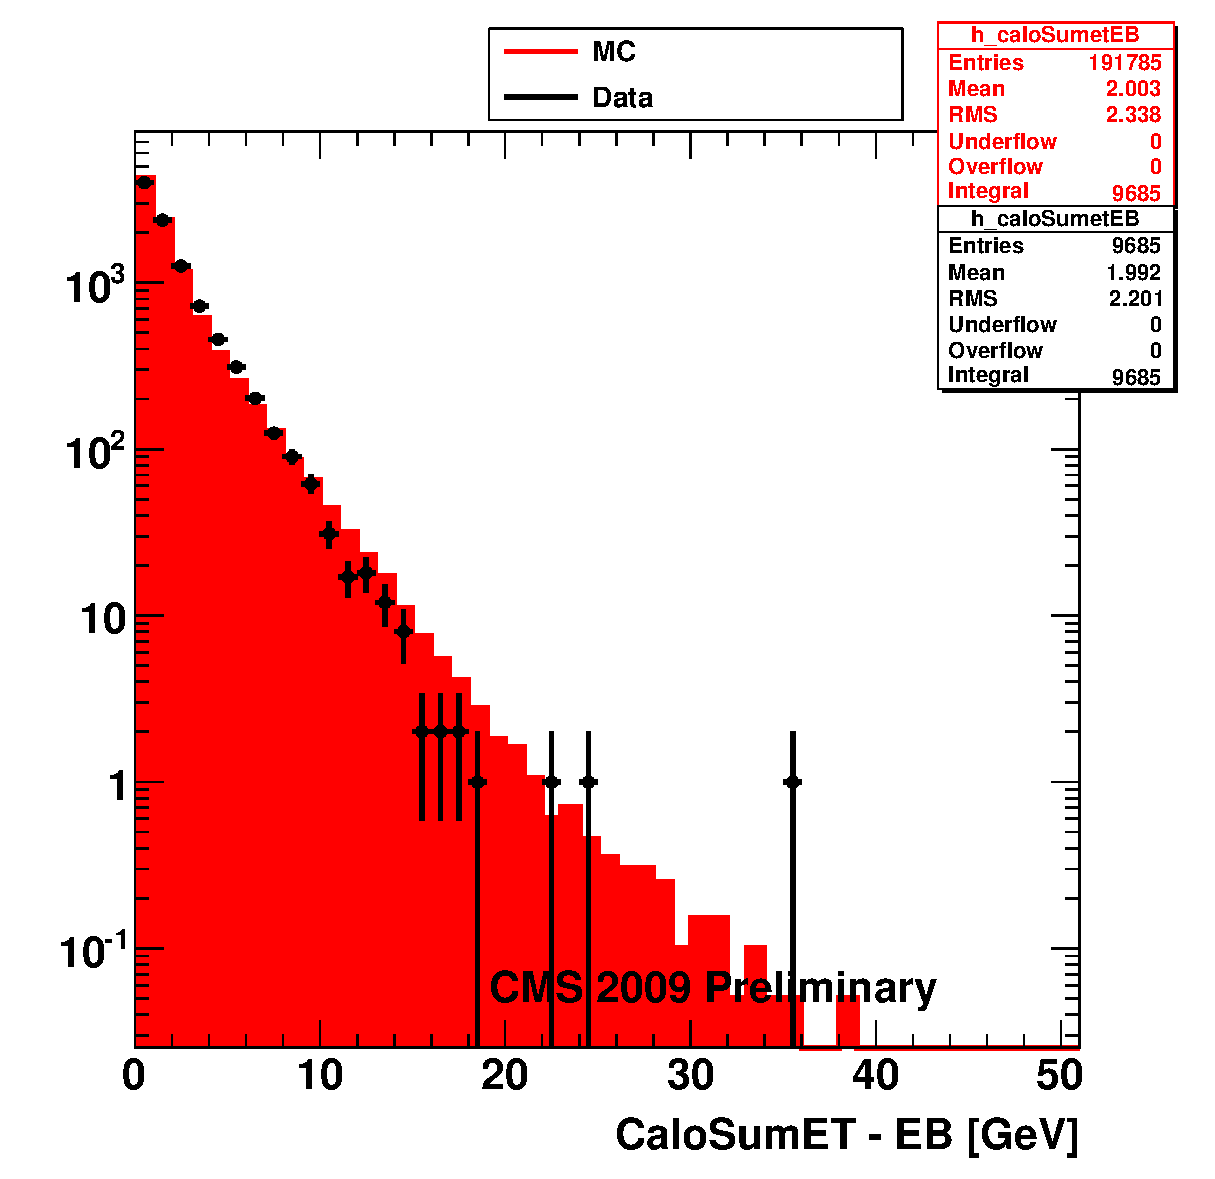
\includegraphics[width=0.40\textwidth]{plots_DataVsMC_MB_2360GeV/h_caloSumetEB.eps} \\
 \end{tabular}
\caption{SumET in ECAL barrel in 2360 GeV data compared
   with Monte Carlo simulation. Same distribution is shown in linear (left) and log (right) scales
   \label{fig:DataVsMC_MB_2360_5}}
\end{figure}

\begin{figure}[h!]
 \centering
 \begin{tabular}{ll}
  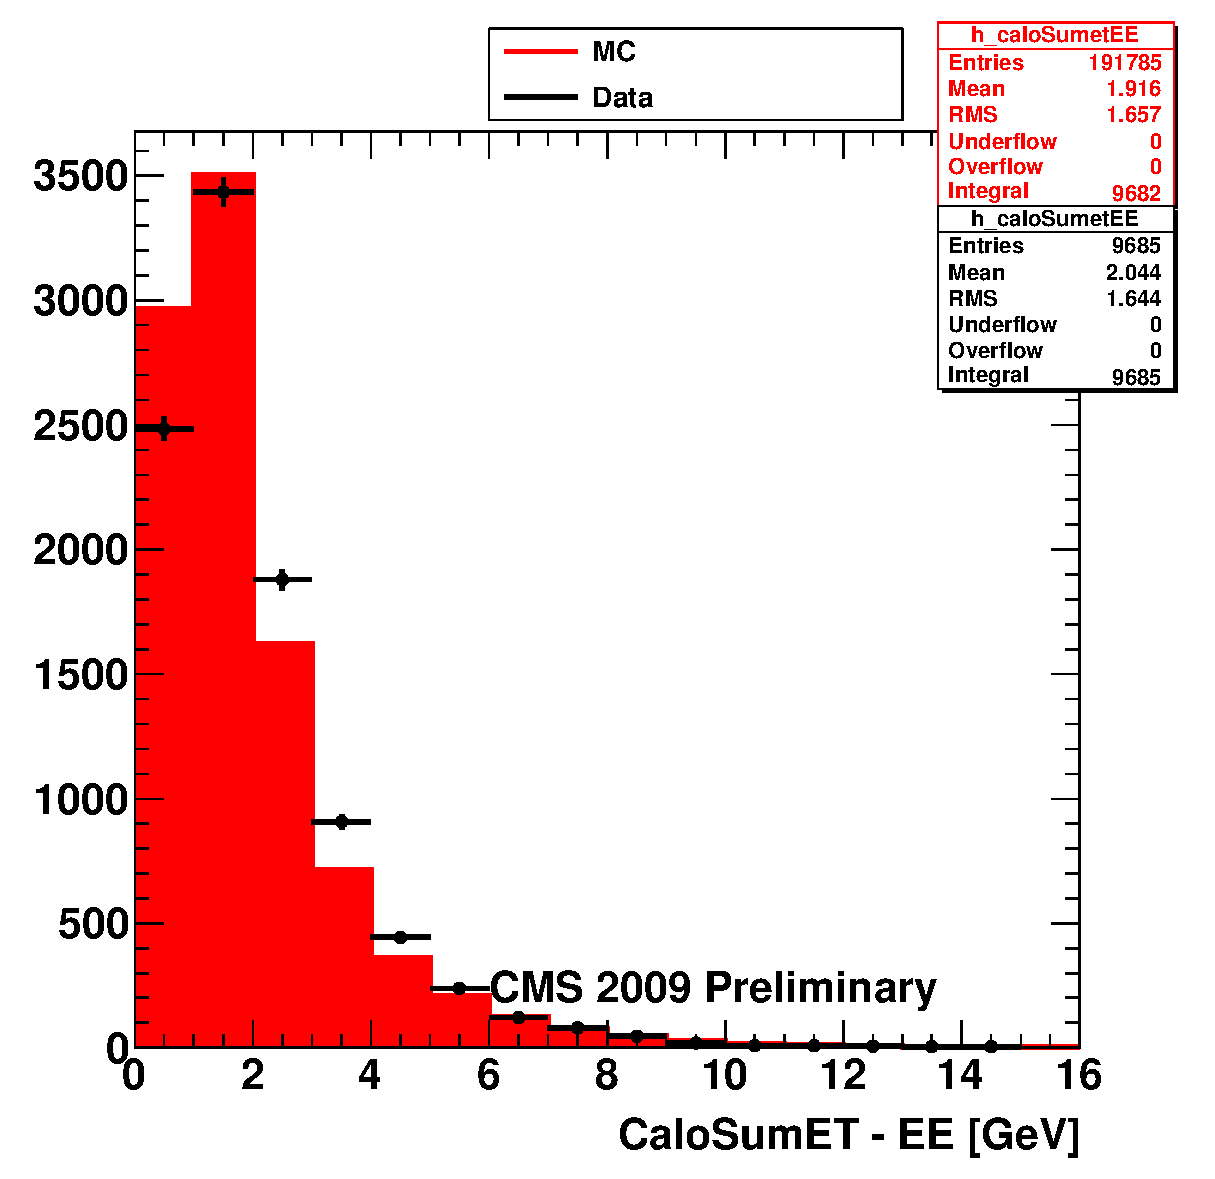
\includegraphics[width=0.40\textwidth]{plots_DataVsMC_MB_2360GeV/h_caloSumetEE_lin.eps} &
  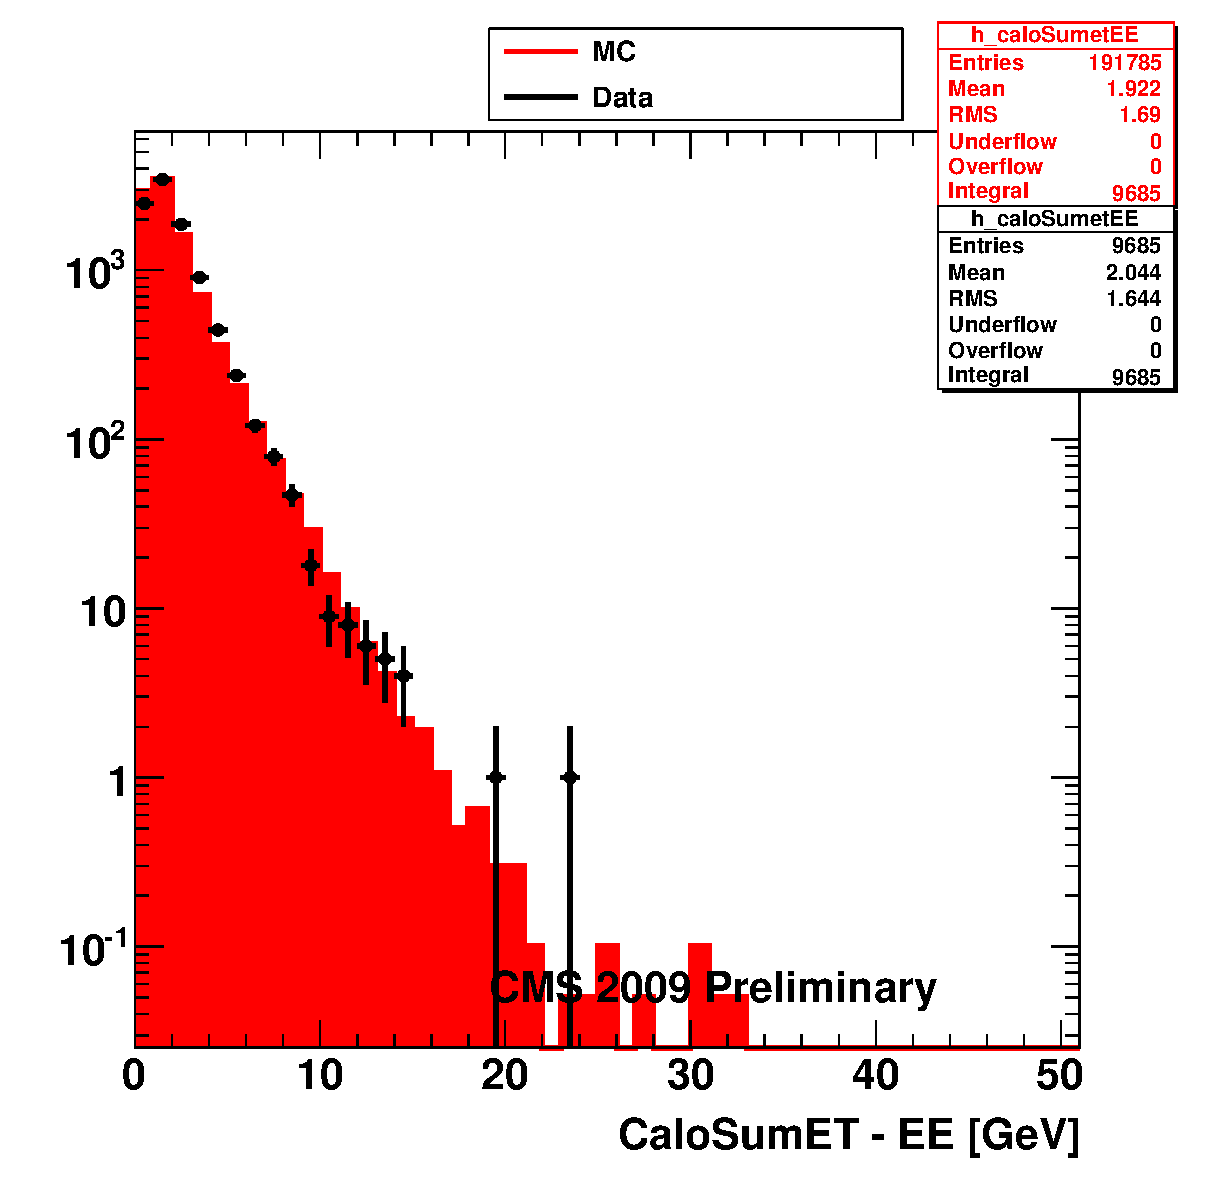
\includegraphics[width=0.40\textwidth]{plots_DataVsMC_MB_2360GeV/h_caloSumetEE.eps} \\
 \end{tabular}
\caption{SumET in ECAL endcap in 2360 GeV data compared
   with Monte Carlo simulation. Same distribution is shown in linear (left) and log (right) scales
         \label{fig:DataVsMC_MB_2360_6}}
\end{figure}

\begin{figure}[h!]
 \centering
 \begin{tabular}{ll}
  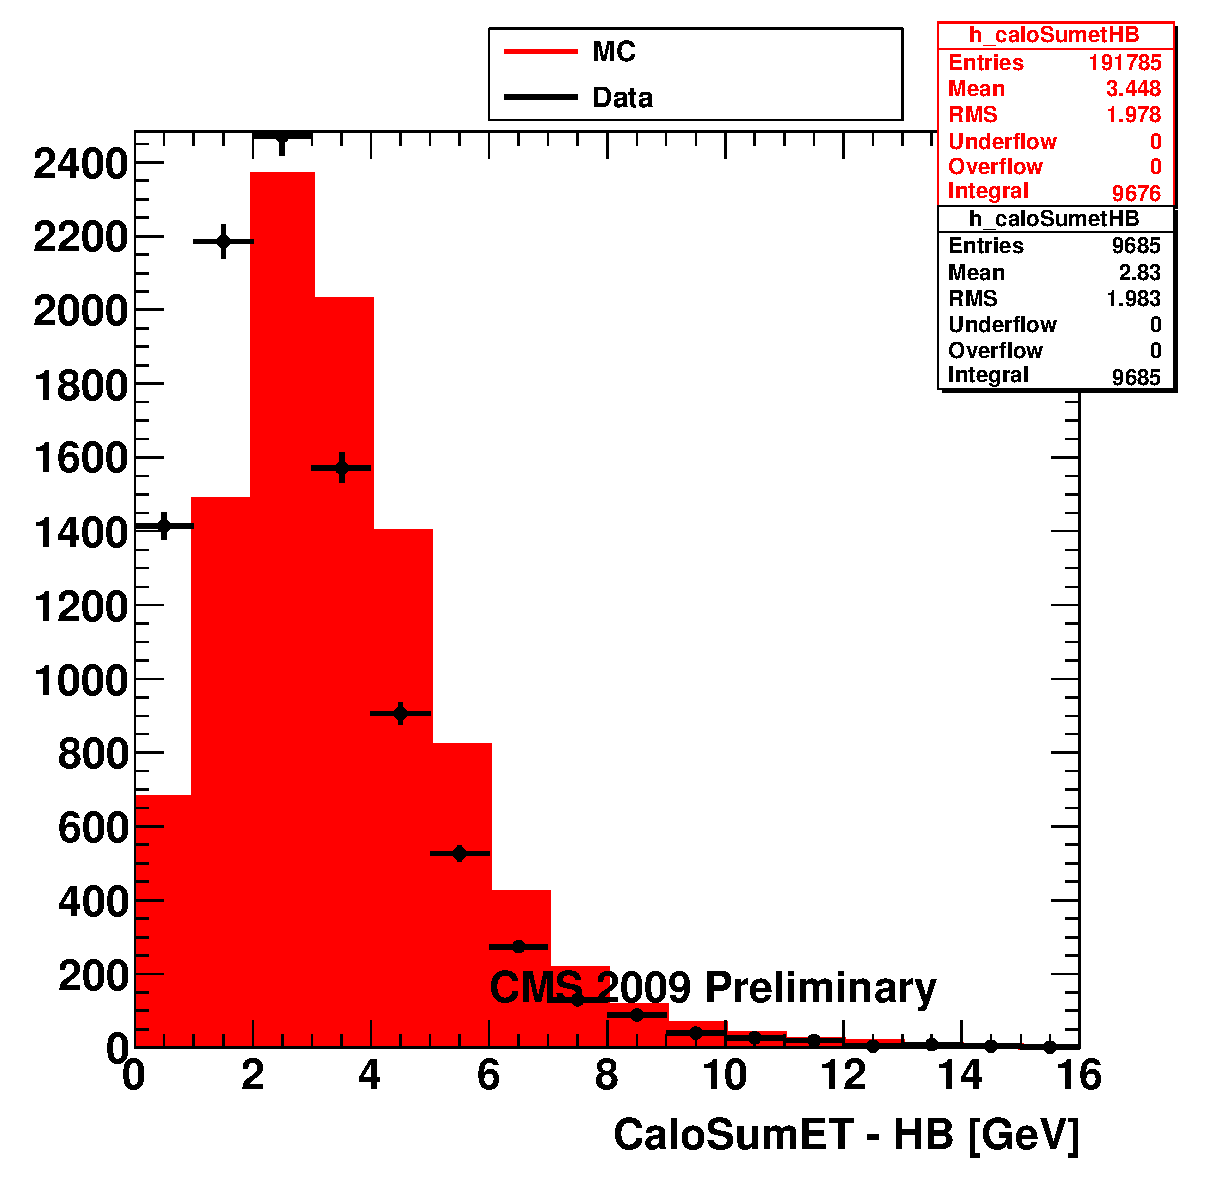
\includegraphics[width=0.40\textwidth]{plots_DataVsMC_MB_2360GeV/h_caloSumetHB_lin.eps} &
  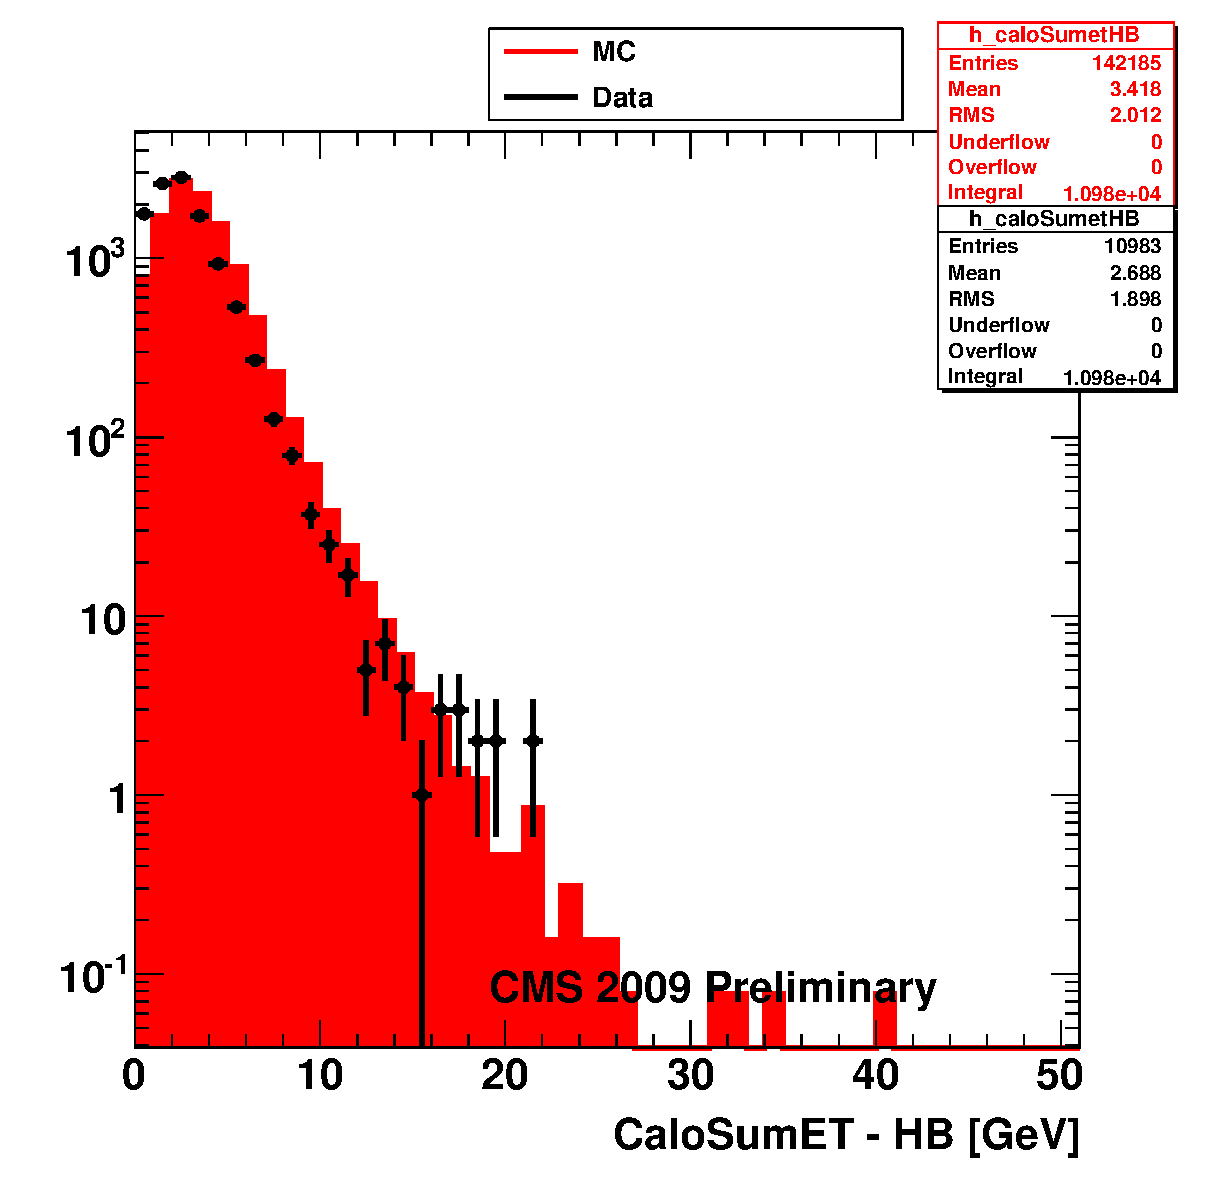
\includegraphics[width=0.40\textwidth]{plots_DataVsMC_MB_2360GeV/h_caloSumetHB.eps} \\
 \end{tabular}
 \caption{SumET in HCAL barrel in 2360 GeV data compared
   with Monte Carlo simulation. Same distribution is shown in linear (left) and log (right) scales
          \label{fig:DataVsMC_MB_2360_7}}
\end{figure}

\begin{figure}[h!]
 \centering
 \begin{tabular}{ll}
  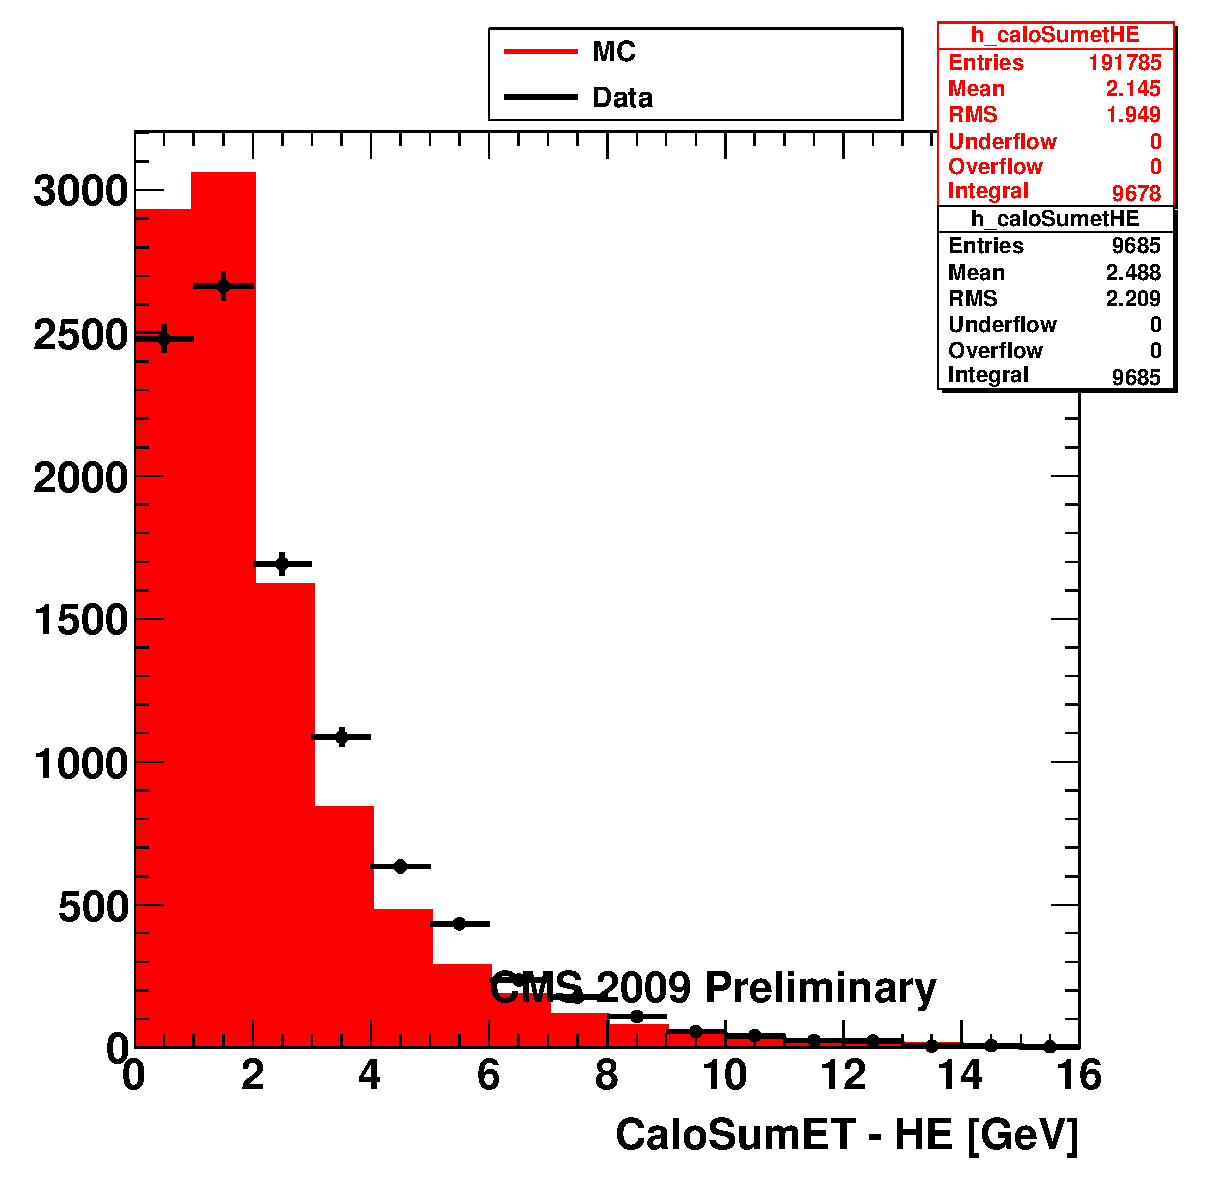
\includegraphics[width=0.40\textwidth]{plots_DataVsMC_MB_2360GeV/h_caloSumetHE_lin.eps} &
  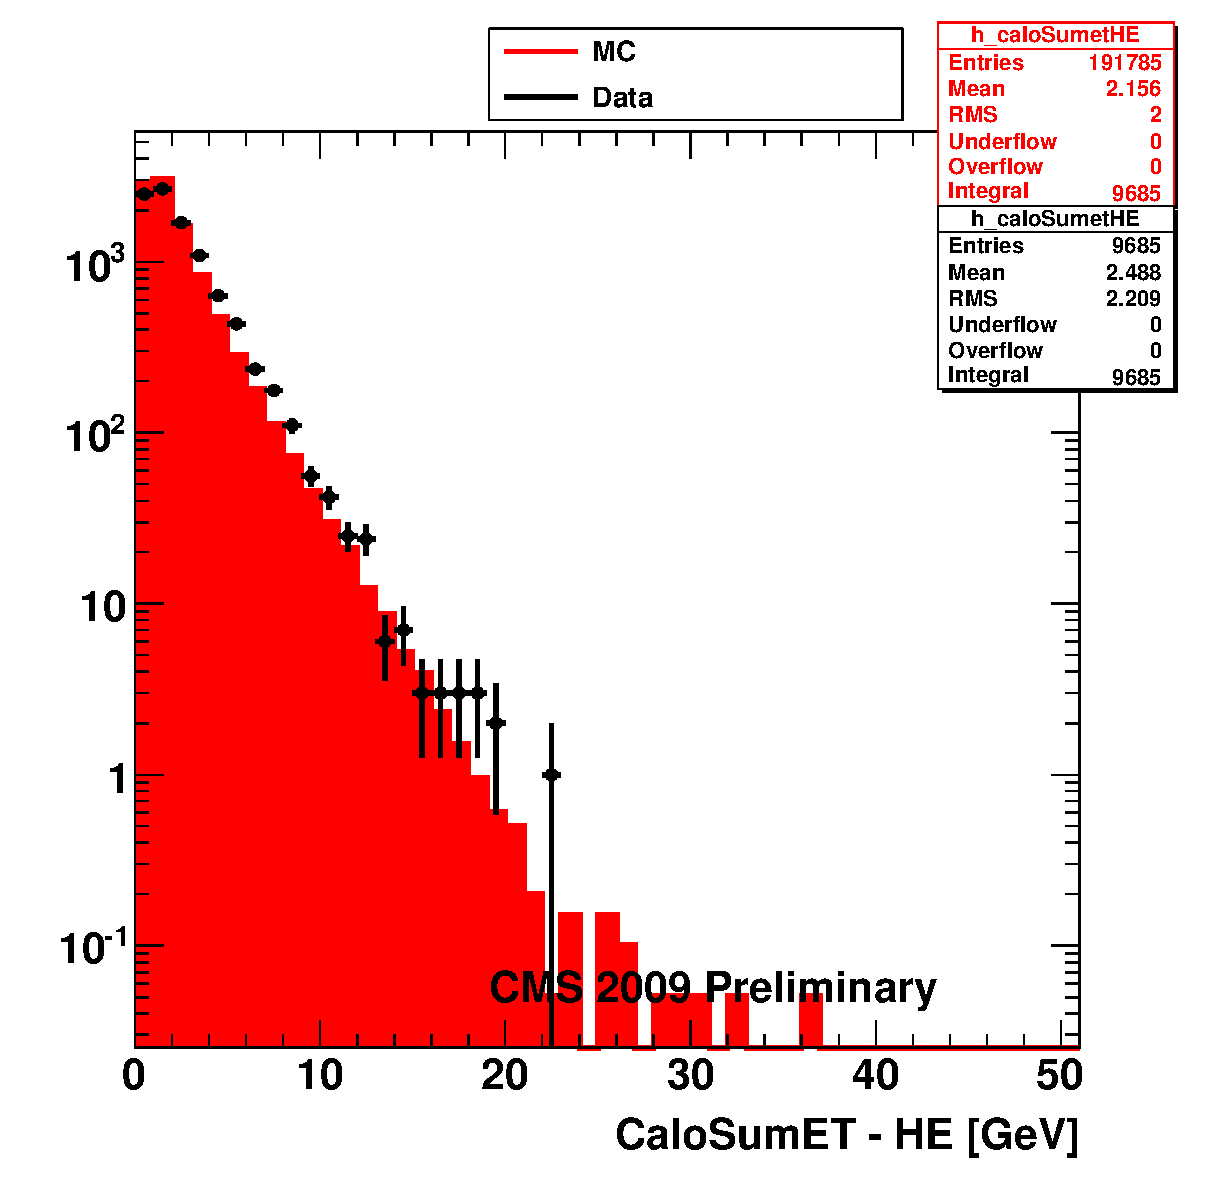
\includegraphics[width=0.40\textwidth]{plots_DataVsMC_MB_2360GeV/h_caloSumetHE.eps} \\
 \end{tabular}
 \caption{SumET in HCAL endcap in 2360 GeV data compared
   with Monte Carlo simulation. Same distribution is shown in linear (left) and log (right) scales
          \label{fig:DataVsMC_MB_2360_8}}
\end{figure}

\begin{figure}[h!]
 \centering
 \begin{tabular}{ll}
  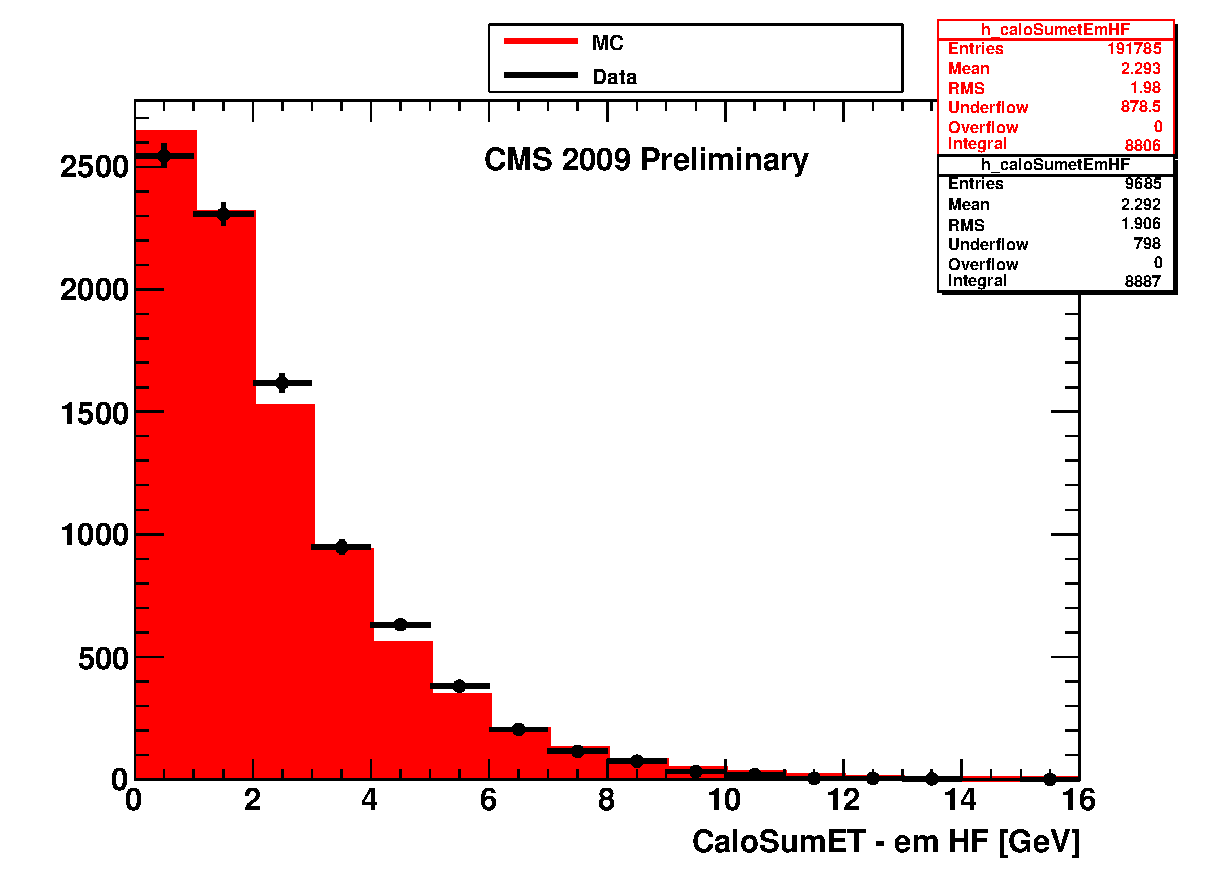
\includegraphics[width=0.40\textwidth]{plots_DataVsMC_MB_2360GeV/h_caloSumetEmHF_lin.eps} &
  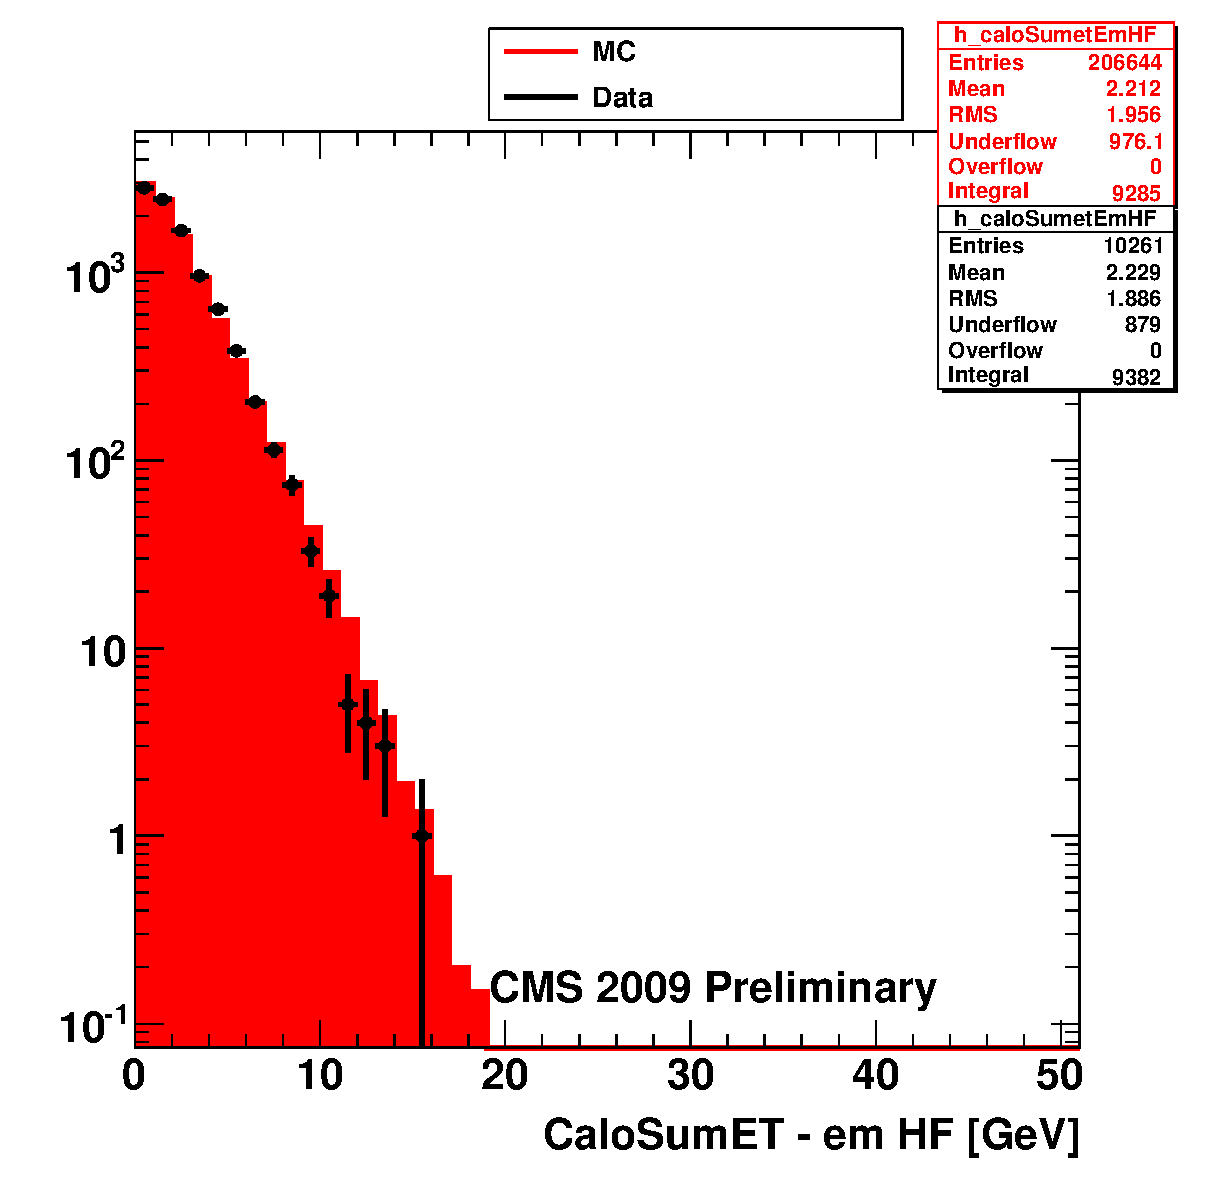
\includegraphics[width=0.40\textwidth]{plots_DataVsMC_MB_2360GeV/h_caloSumetEmHF.eps} \\
 \end{tabular}
 \caption{SumET in HF in electromagnetic part in 2360 GeV data compared
   with Monte Carlo simulation. Same distribution is shown in linear (left) and log (right) scales
          \label{fig:DataVsMC_MB_2360_9}}
\end{figure}

\begin{figure}[h!]
 \centering
 \begin{tabular}{ll}
  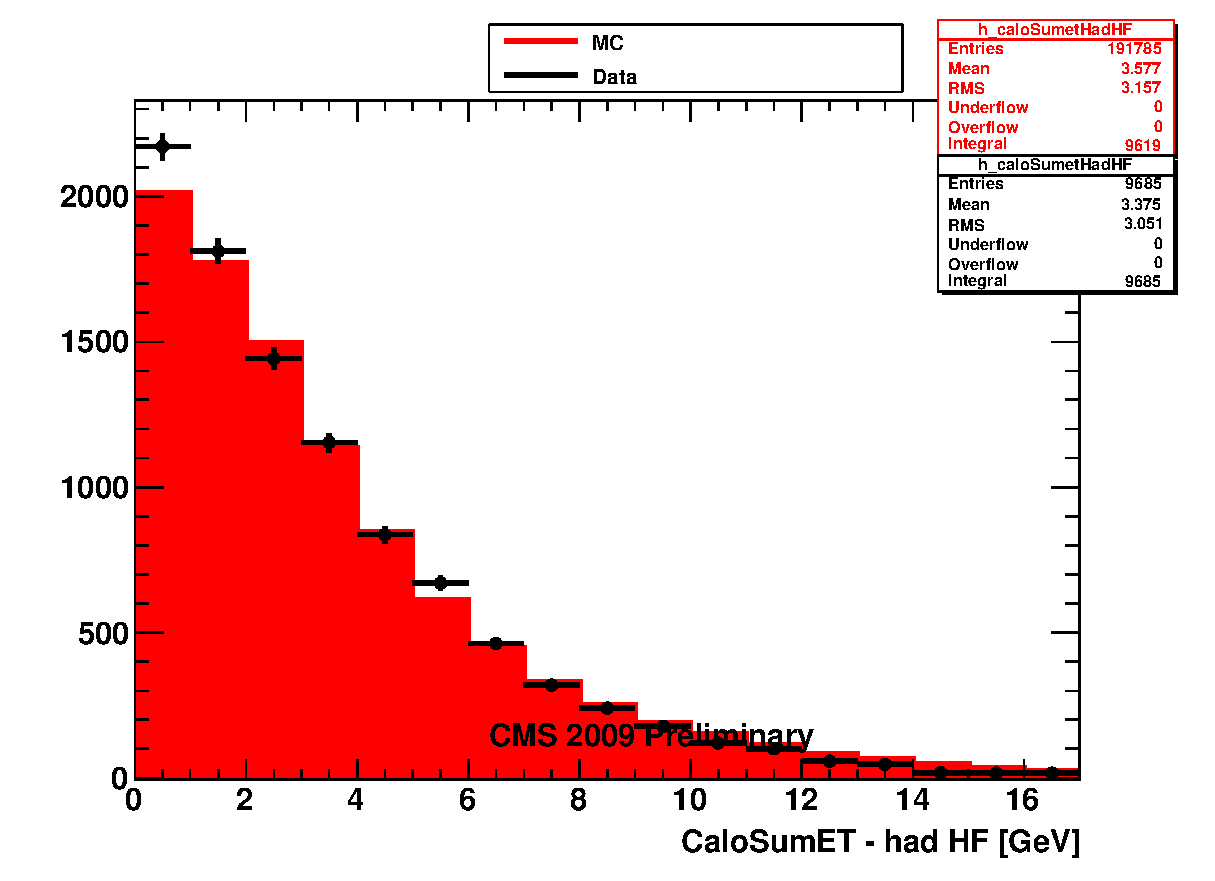
\includegraphics[width=0.40\textwidth]{plots_DataVsMC_MB_2360GeV/h_caloSumetHadHF_lin.eps} &
  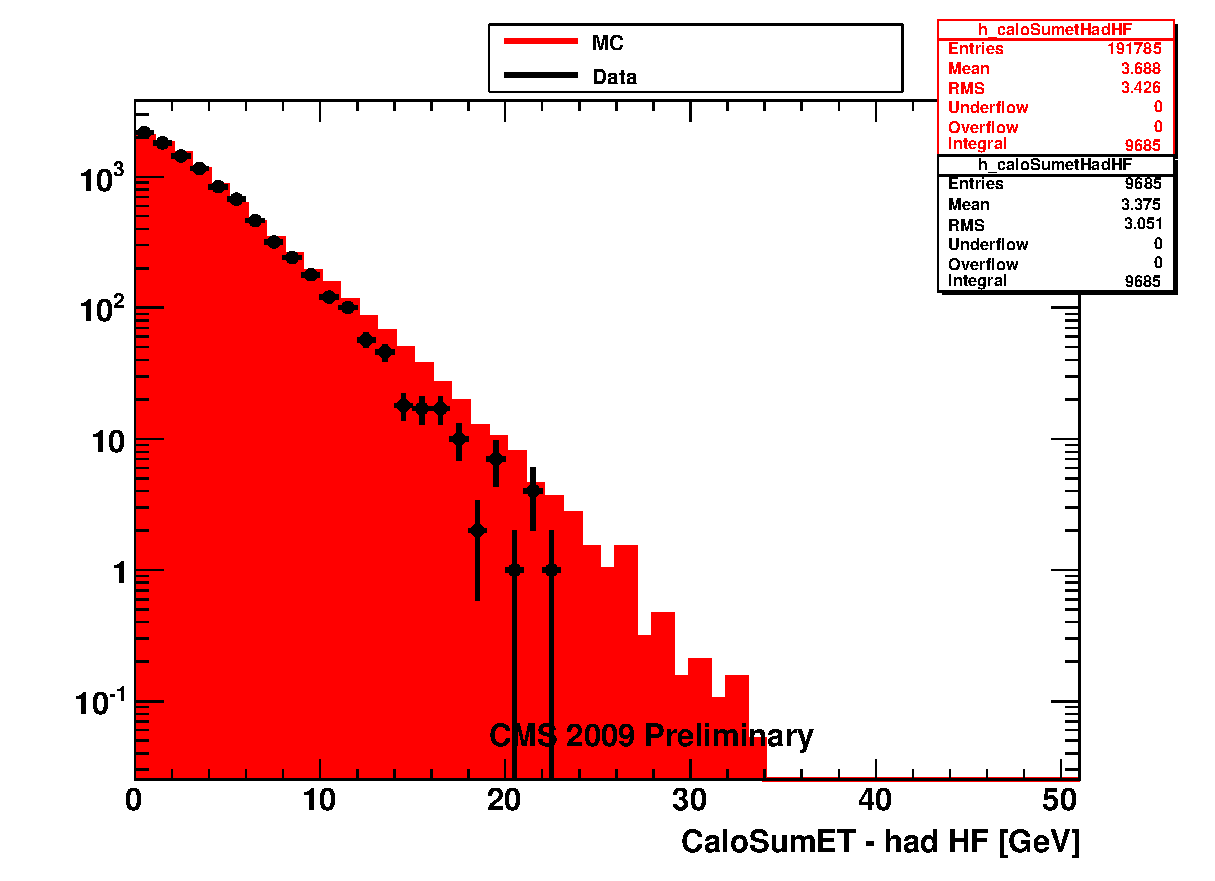
\includegraphics[width=0.40\textwidth]{plots_DataVsMC_MB_2360GeV/h_caloSumetHadHF.eps} \\
 \end{tabular}
 \caption{SumET in HF in hadronic part in 2360 GeV data compared
   with Monte Carlo simulation. Same distribution is shown in linear (left) and log (right) scales
          \label{fig:DataVsMC_MB_2360_10}}
\end{figure}

\begin{figure}[h!]
 \centering
  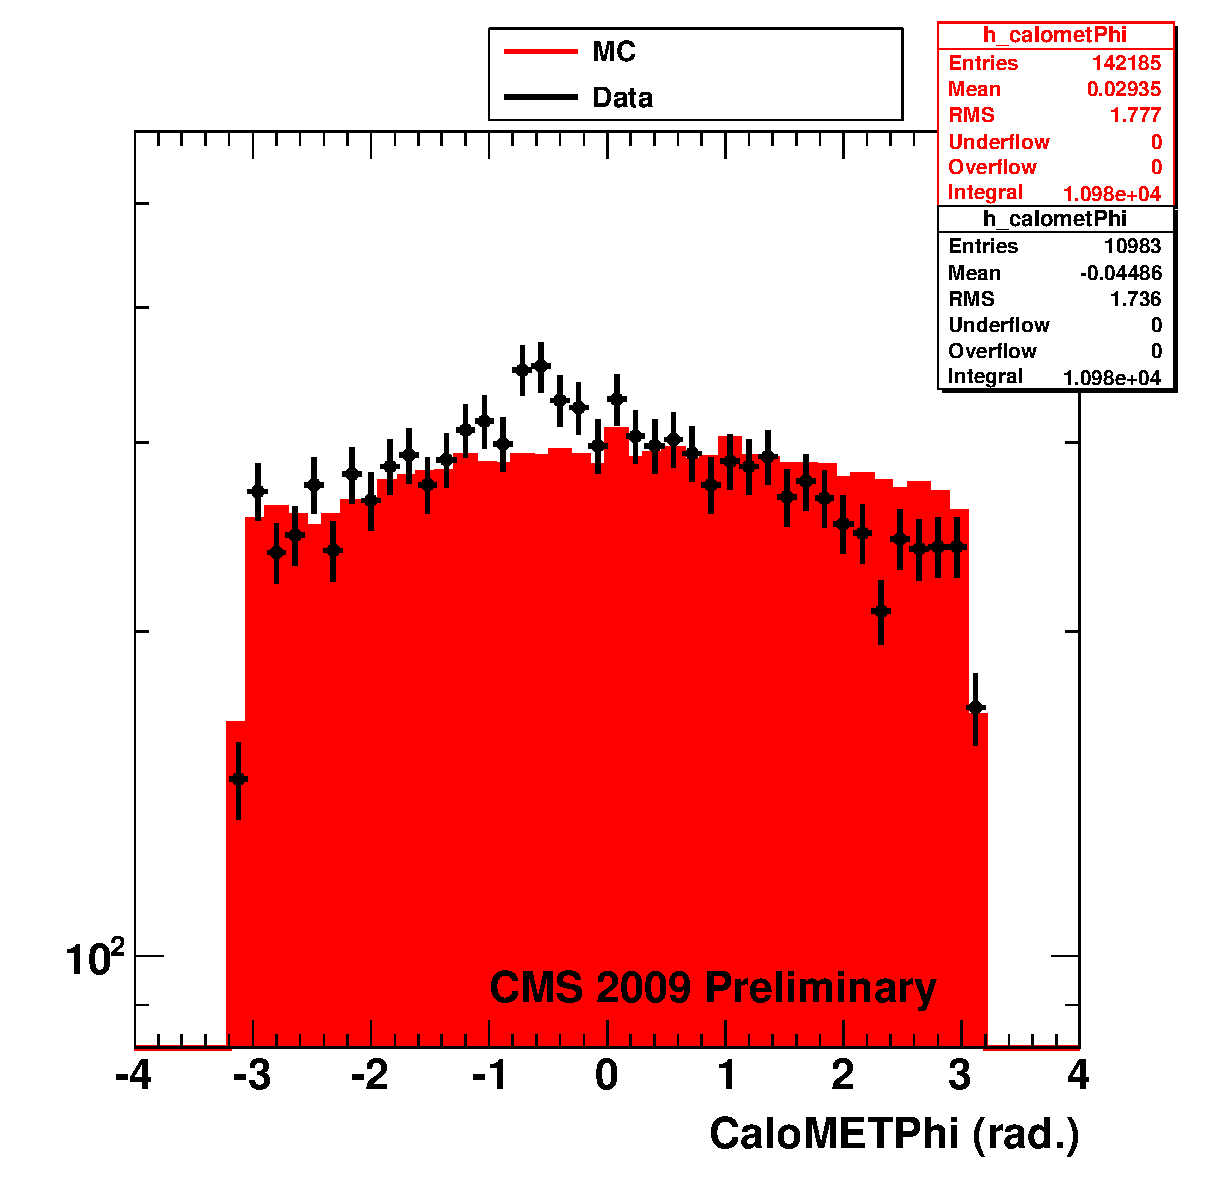
\includegraphics[width=0.40\textwidth]{plots_DataVsMC_MB_2360GeV/h_calometPhi.eps}
 \caption{$\phi_{\etmiss}$ distributions in 2360 GeV data compared
   with Monte Carlo simulation.
          \label{fig:DataVsMC_MB_2360_11}}
\end{figure}

\begin{figure}[h!]
 \centering
 \begin{tabular}{ll}
  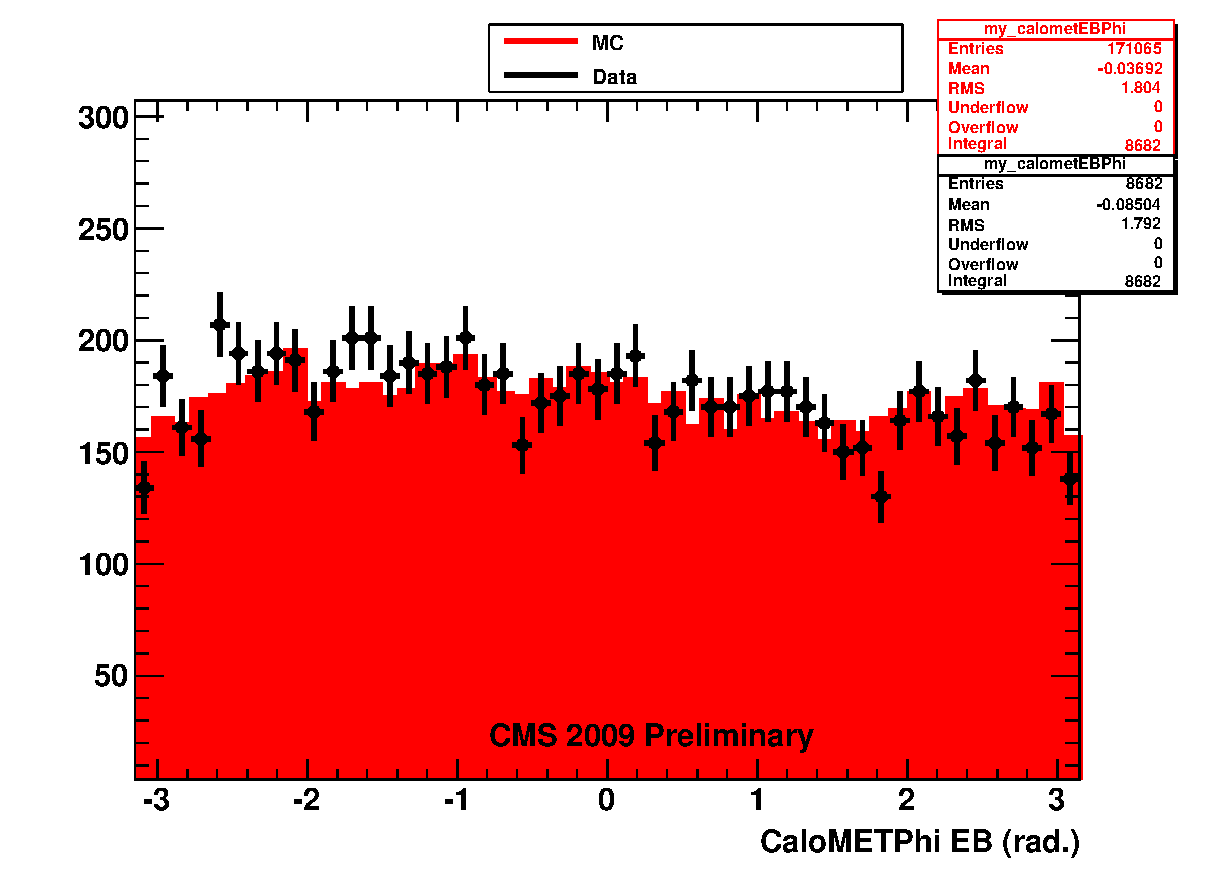
\includegraphics[width=0.40\textwidth]{plots_DataVsMC_MB_2360GeV/my_calometEBPhi_lin.eps} &
  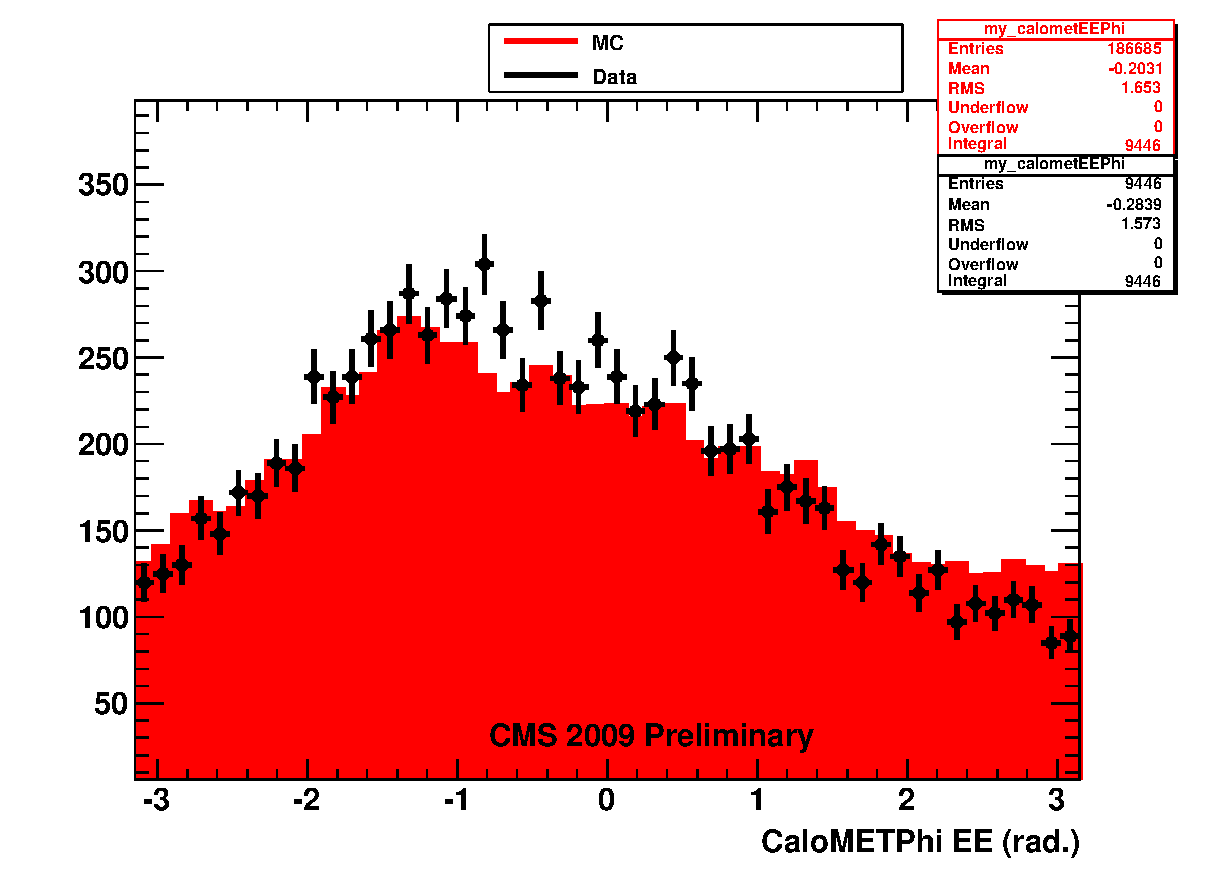
\includegraphics[width=0.40\textwidth]{plots_DataVsMC_MB_2360GeV/my_calometEEPhi_lin.eps} \\
 \end{tabular}
 \caption{$\phi_{\etmiss}$ distributions in ECAL barrel and endcap in 2360 GeV data compared
   with Monte Carlo simulation.
          \label{fig:DataVsMC_MB_2360_12}}
\end{figure}

\begin{figure}[h!]
 \centering
 \begin{tabular}{ll}
  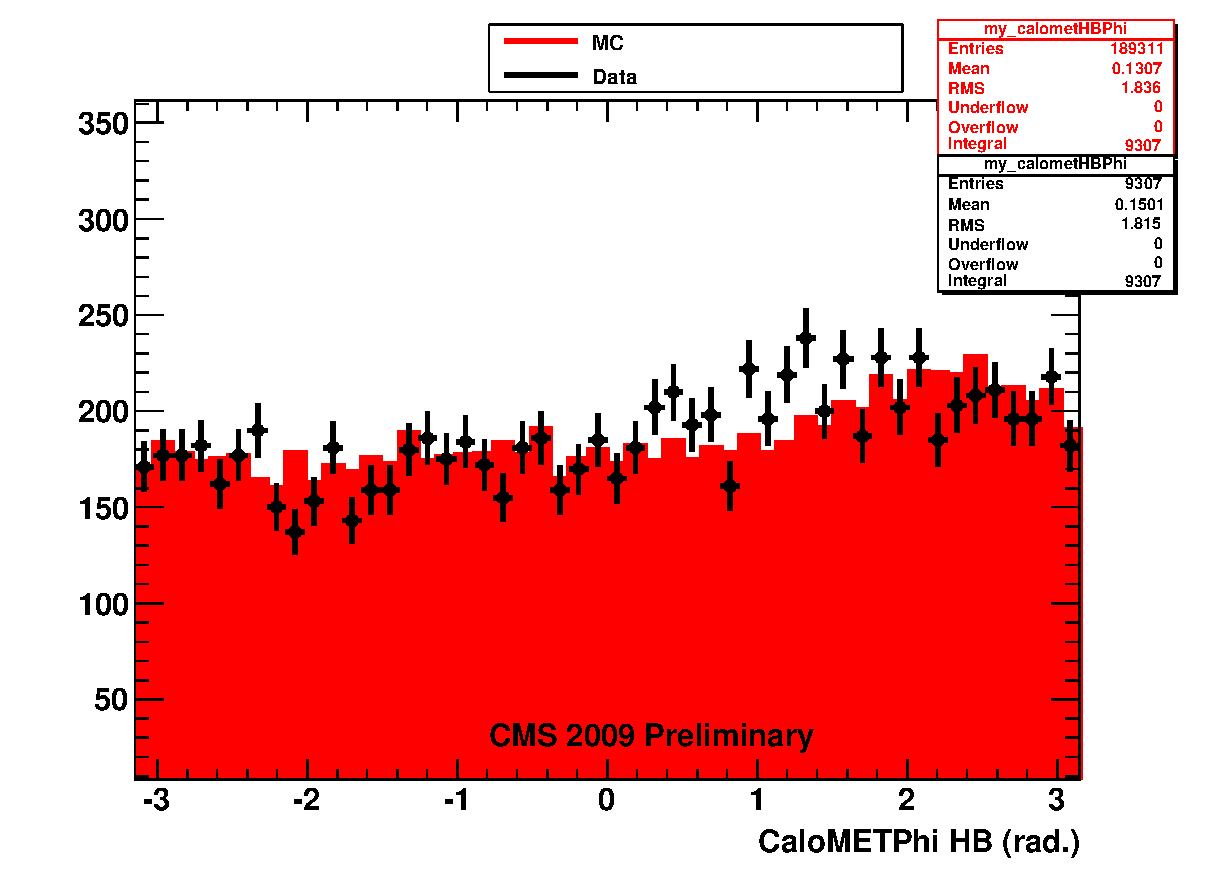
\includegraphics[width=0.40\textwidth]{plots_DataVsMC_MB_2360GeV/my_calometHBPhi_lin.eps} &
  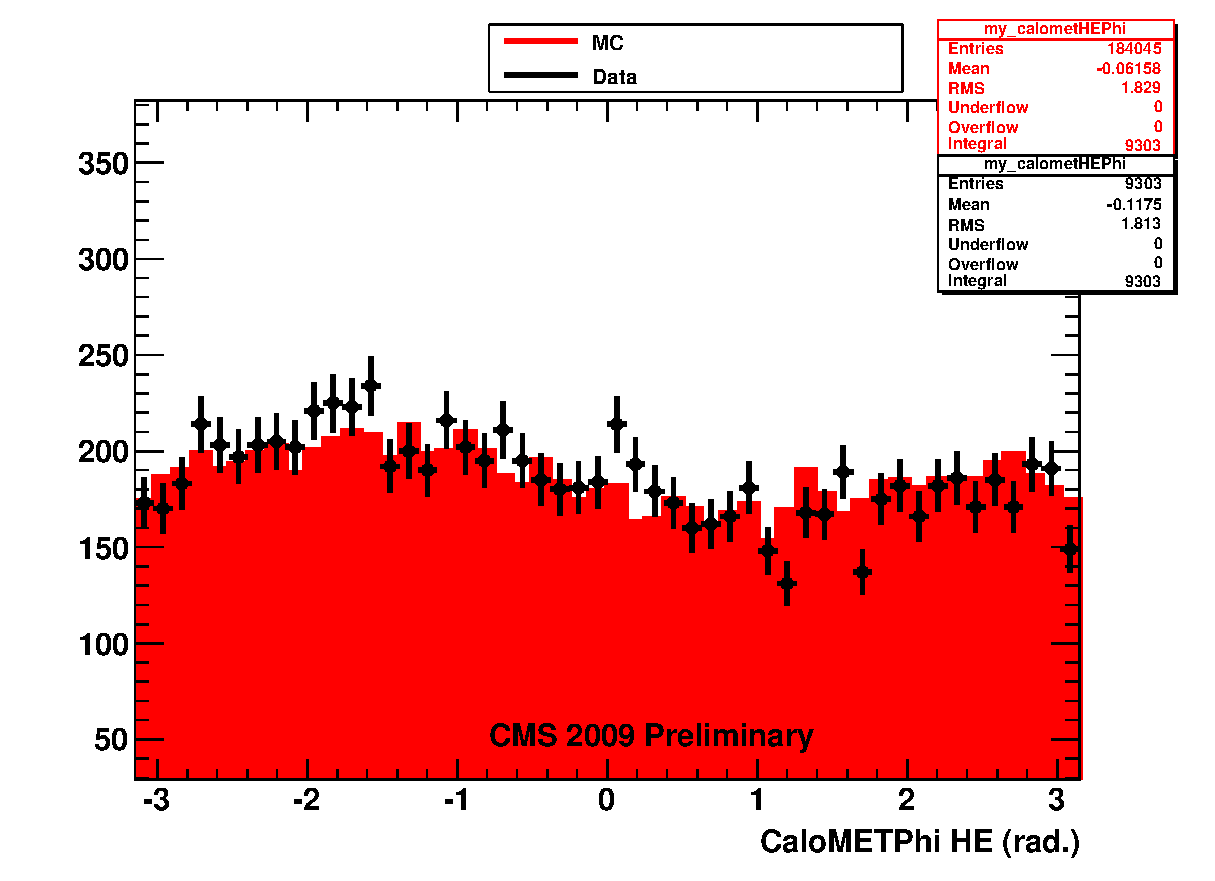
\includegraphics[width=0.40\textwidth]{plots_DataVsMC_MB_2360GeV/my_calometHEPhi_lin.eps} \\
 \end{tabular}
 \caption{$\phi_{\etmiss}$ distributions in HCAL barrel and endcap in 2360 GeV data compared
   with Monte Carlo simulation.
          \label{fig:DataVsMC_MB_2360_13}}
\end{figure}

\begin{figure}[h!]
 \centering
 \begin{tabular}{ll}
  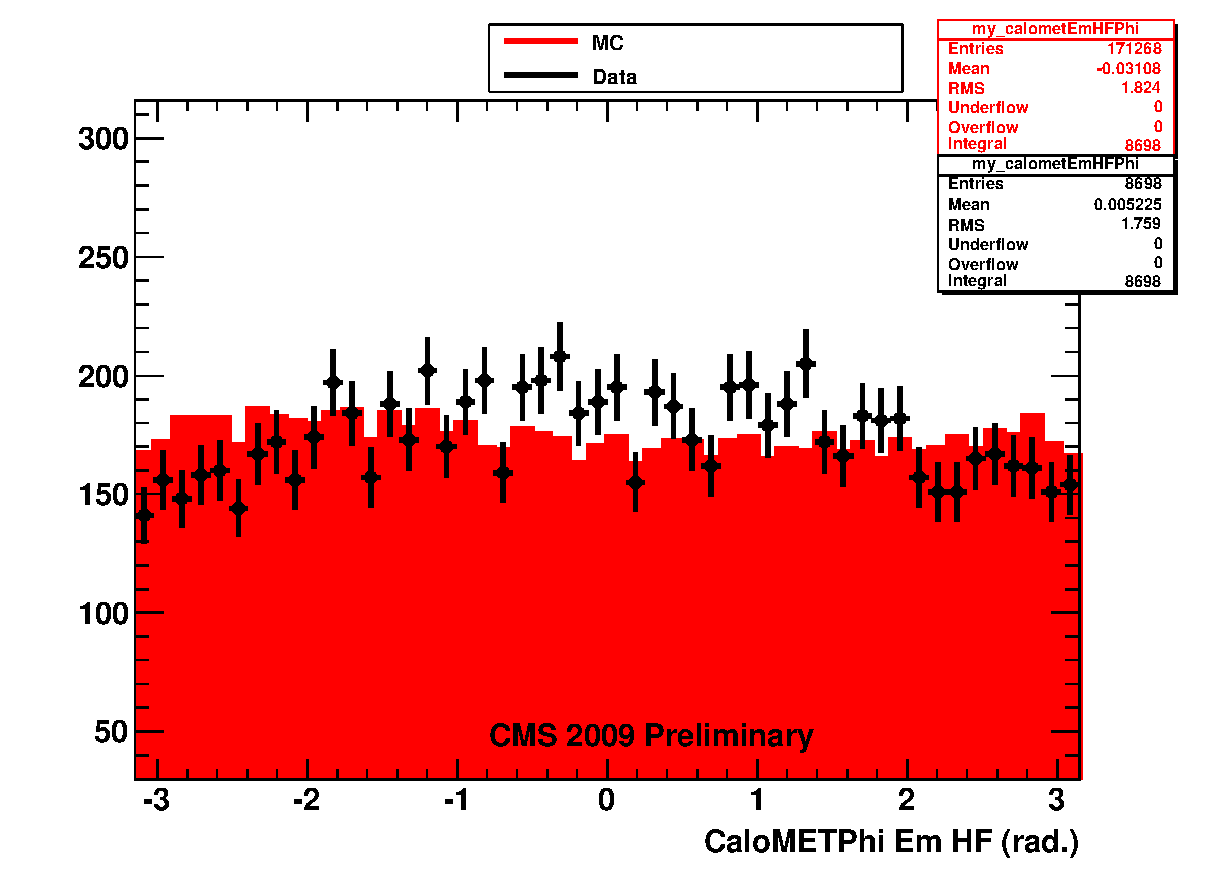
\includegraphics[width=0.40\textwidth]{plots_DataVsMC_MB_2360GeV/my_calometEmHFPhi_lin.eps} &
  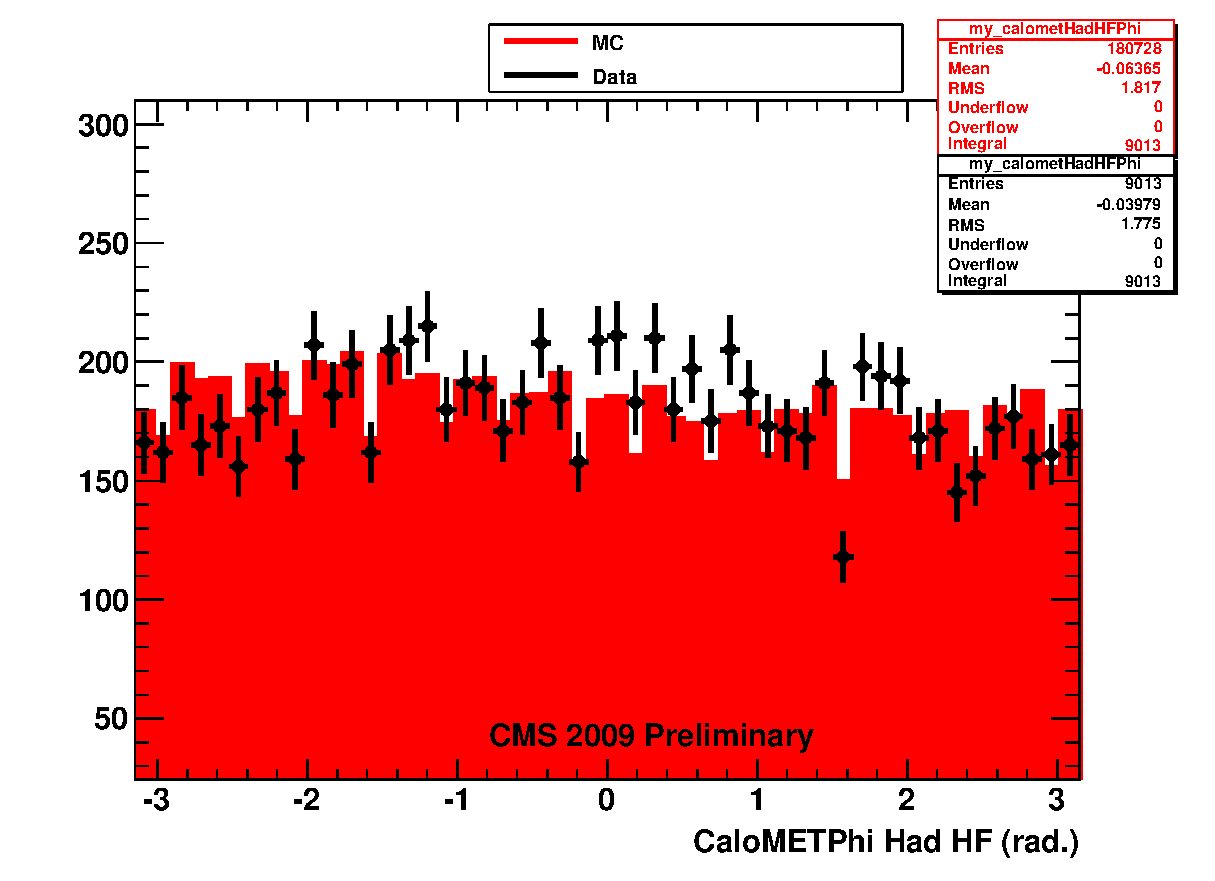
\includegraphics[width=0.40\textwidth]{plots_DataVsMC_MB_2360GeV/my_calometHadHFPhi_lin.eps} \\
 \end{tabular}
 \caption{$\phi_{\etmiss}$ distributions in HF in electromagnetic and hadronic parts in 2360 GeV data compared
   with Monte Carlo simulation.
          \label{fig:DataVsMC_MB_2360_14}}
\end{figure}

\clearpage

Some of the features of the $\etmiss>15$~GeV events are listed below,
ordered by decreasing values of reconstructed $\etmiss$:
\begin{itemize}
\item add event
\item etc..
\end{itemize}

\subsection[$\etmiss$ resolution]{$\etmissB$ resolution}

Here we present the same $\etmiss$ resolution analysis as the one presented in Section~\ref{sc:DataVsMCMB900Res}, repeated for the $2360$~GeV data. 
Figure~\ref{fig:MExySigma_vs_SumET_2360} shows the $\sigma\left(\exmiss\right)$ and $\sigma\left(\eymiss\right)$ 
vs. $\sum E_\text{T}$ for 2360 GeV data compared with Monte Carlo simulation. Figures~\ref{fig:MExSigma_vs_SumET_2360_fit} 
and \ref{fig:MEySigma_vs_SumET_2360_fit} show the fit of $\sigma\left(\exmiss\right)$ and $\sigma\left(\eymiss\right)$ vs. 
$\sum E_\text{T}$ to Eq.~\ref{eq:MET_sigma} for data and  Monte Carlo at $2360$ GeV.

\begin{figure}[h!]
 \centering
 \begin{tabular}{ll}
  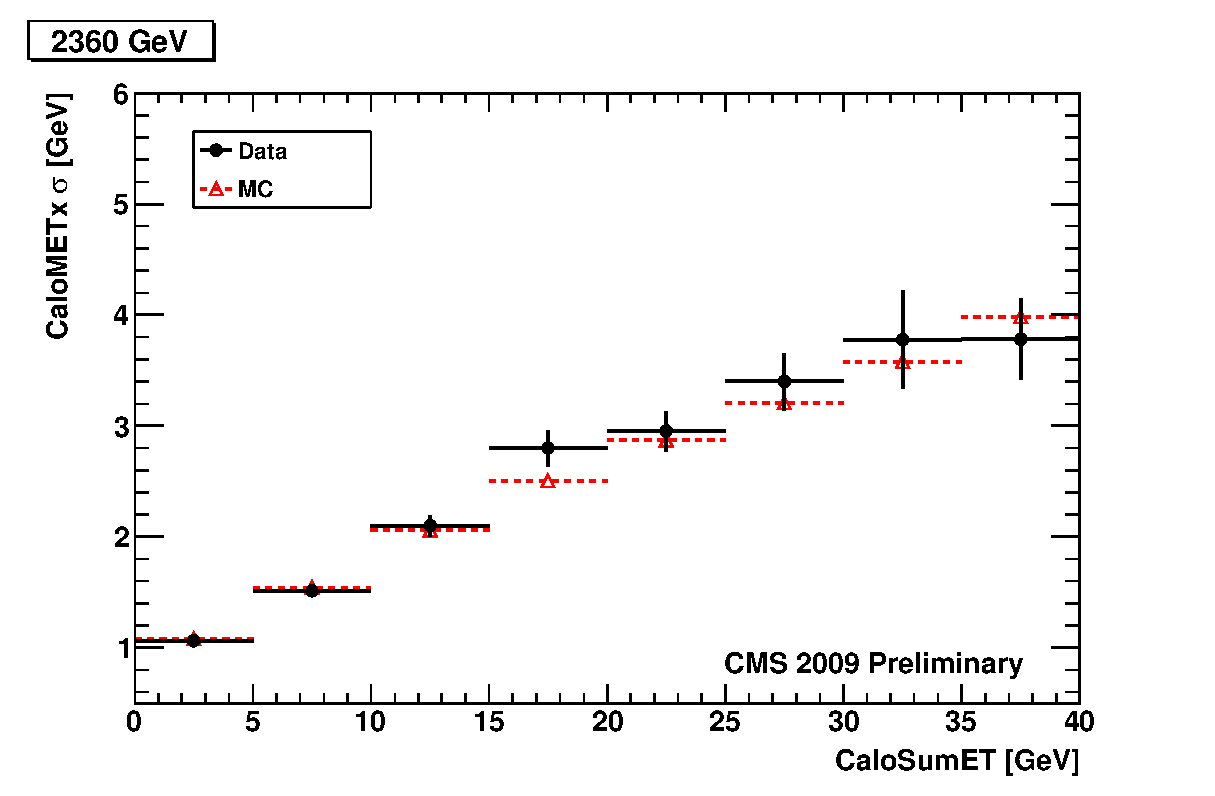
\includegraphics[width=0.5\textwidth]{plots_DataVsMC_MB_2360GeV/h_metxsigma_sumet_2360.eps} &
  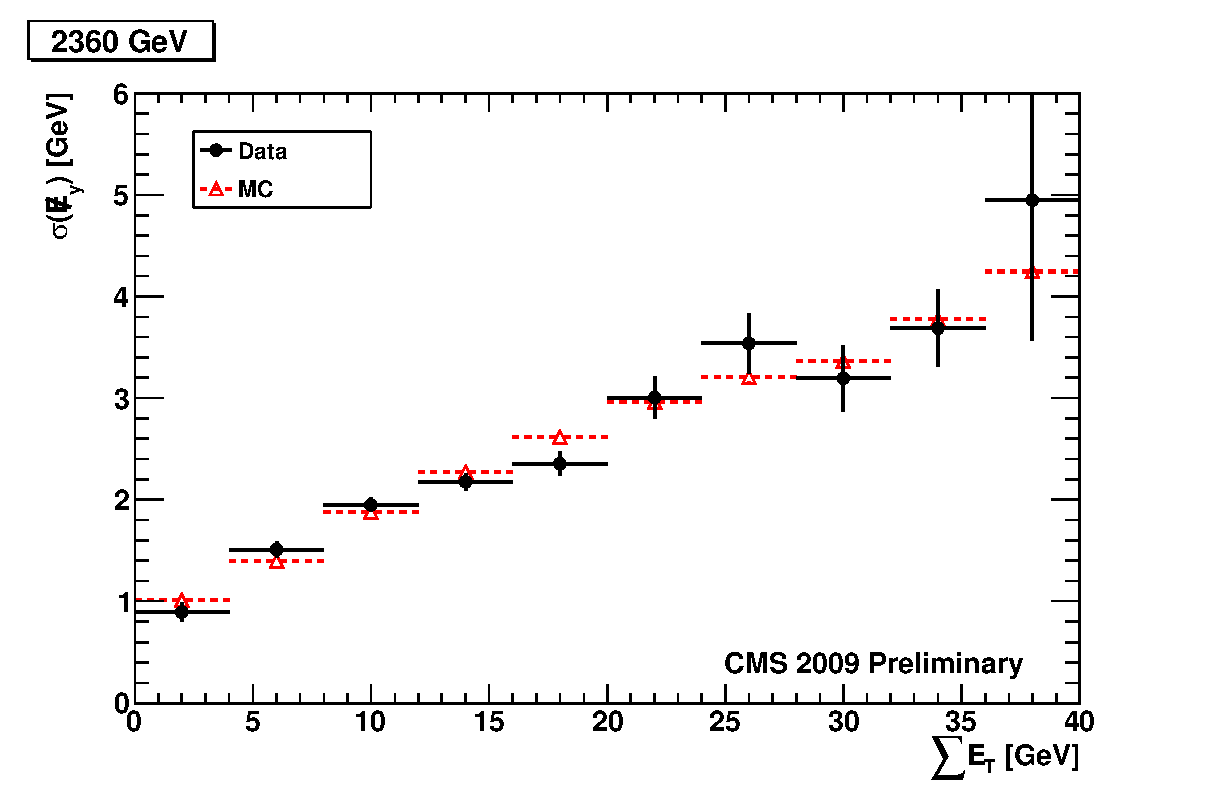
\includegraphics[width=0.5\textwidth]{plots_DataVsMC_MB_2360GeV/h_metysigma_sumet_2360.eps} \\
 \end{tabular}
 \caption{\small $\sigma\left(\exmiss\right)$ and $\sigma\left(\eymiss\right)$ $\sigma$ vs. $\sum E_\text{T}$ for
          data at $2360$ TeV compared with Monte Carlo simulation.\label{fig:MExySigma_vs_SumET_2360}}
\end{figure}

\begin{figure}[h!]
 \centering
 \begin{tabular}{ll}
  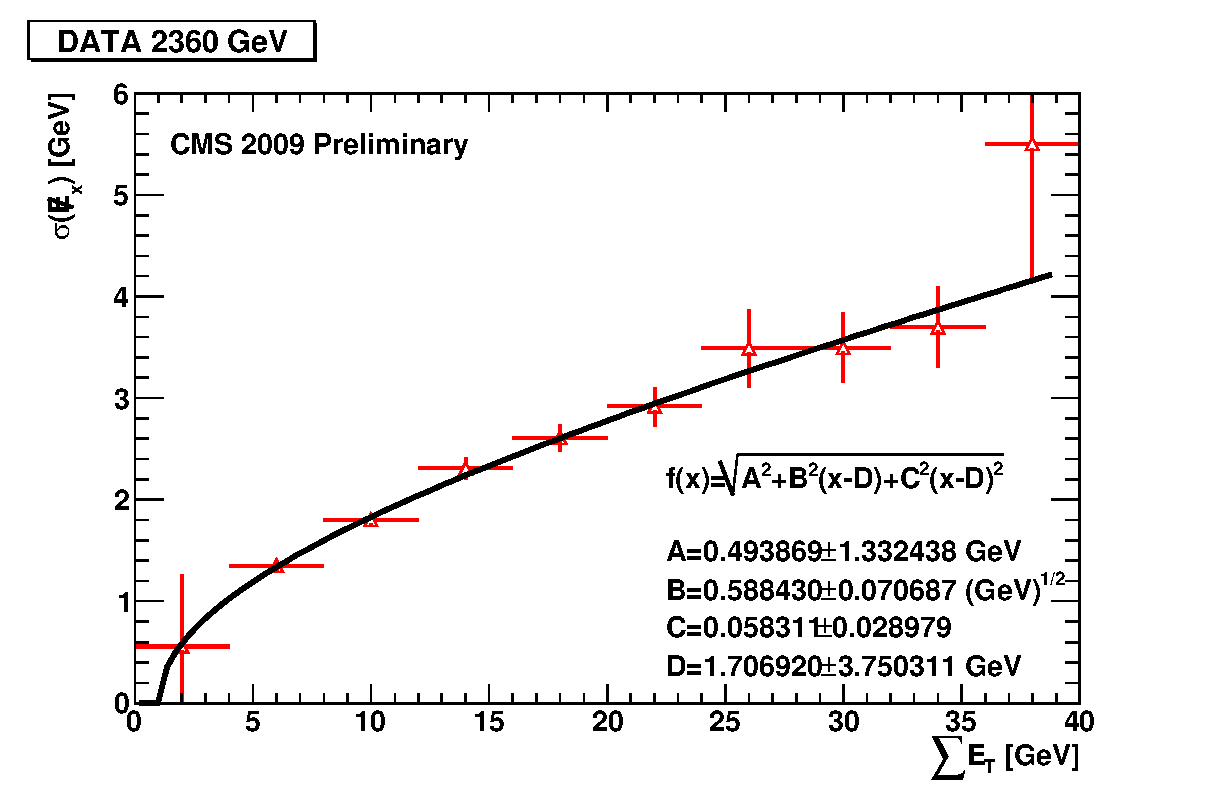
\includegraphics[width=0.5\textwidth]{plots_DataVsMC_MB_2360GeV/final_metxsigma_sumet_DATA_2360.eps} &
  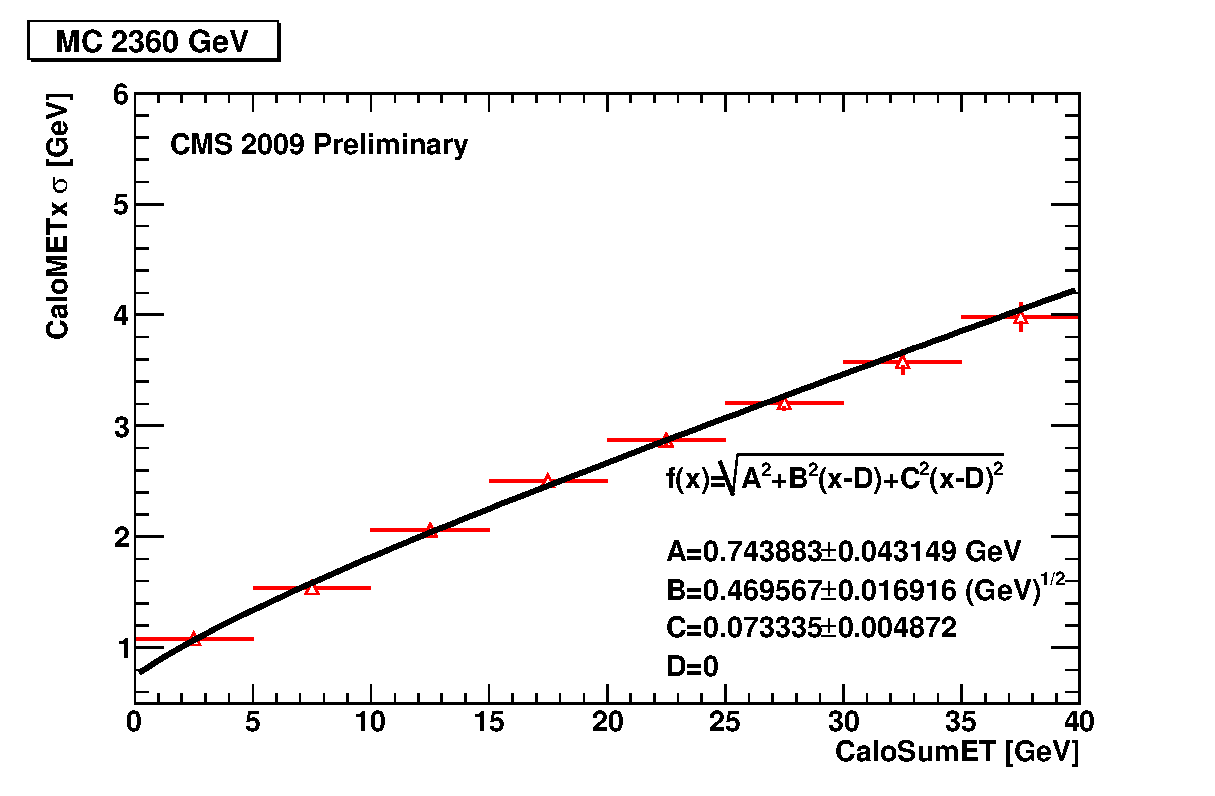
\includegraphics[width=0.5\textwidth]{plots_DataVsMC_MB_2360GeV/final_metxsigma_sumet_MC_2360.eps} \\
 \end{tabular}
 \caption{\small Fit of the $\sigma\left(\exmiss\right)$ vs. $\sum E_\text{T}$ for data and Monte Carlo at $2360$ GeV.\label{fig:MExSigma_vs_SumET_2360_fit}}
\end{figure}

\begin{figure}[h!]
 \centering
 \begin{tabular}{ll}
  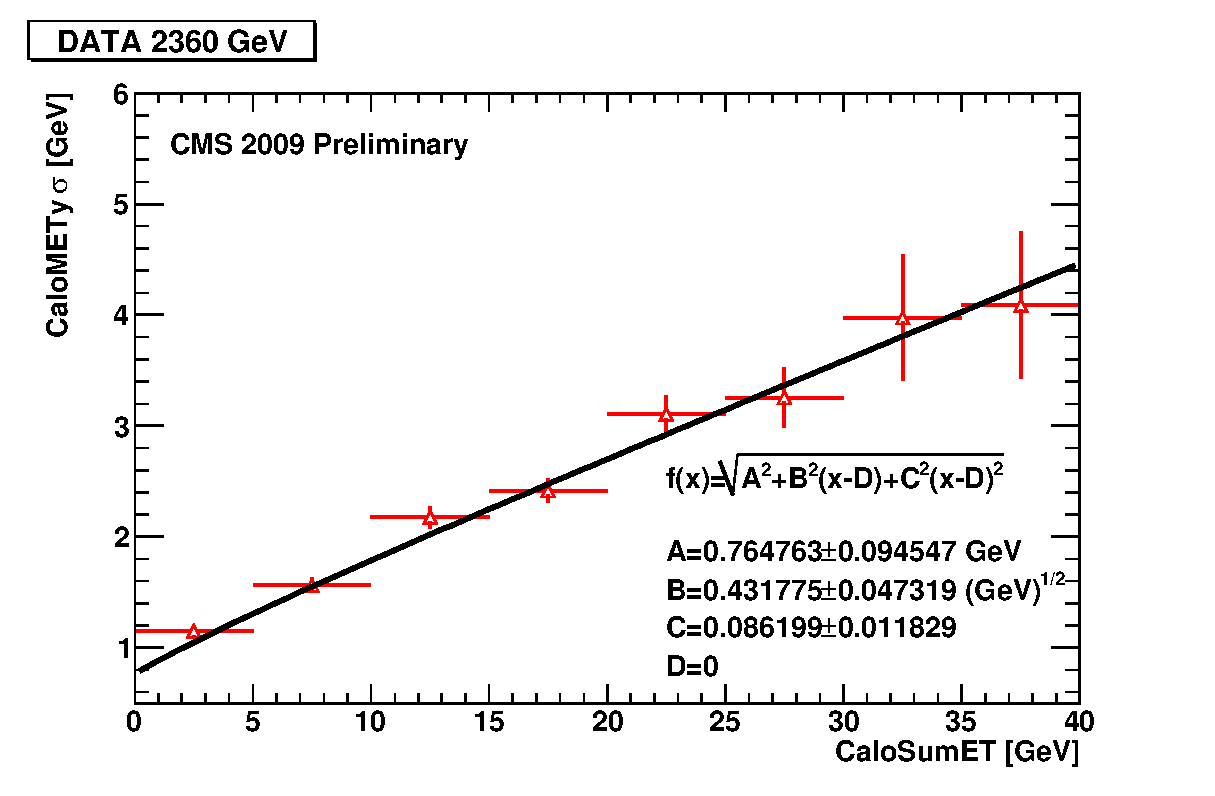
\includegraphics[width=0.5\textwidth]{plots_DataVsMC_MB_2360GeV/final_metysigma_sumet_DATA_2360.eps} &
  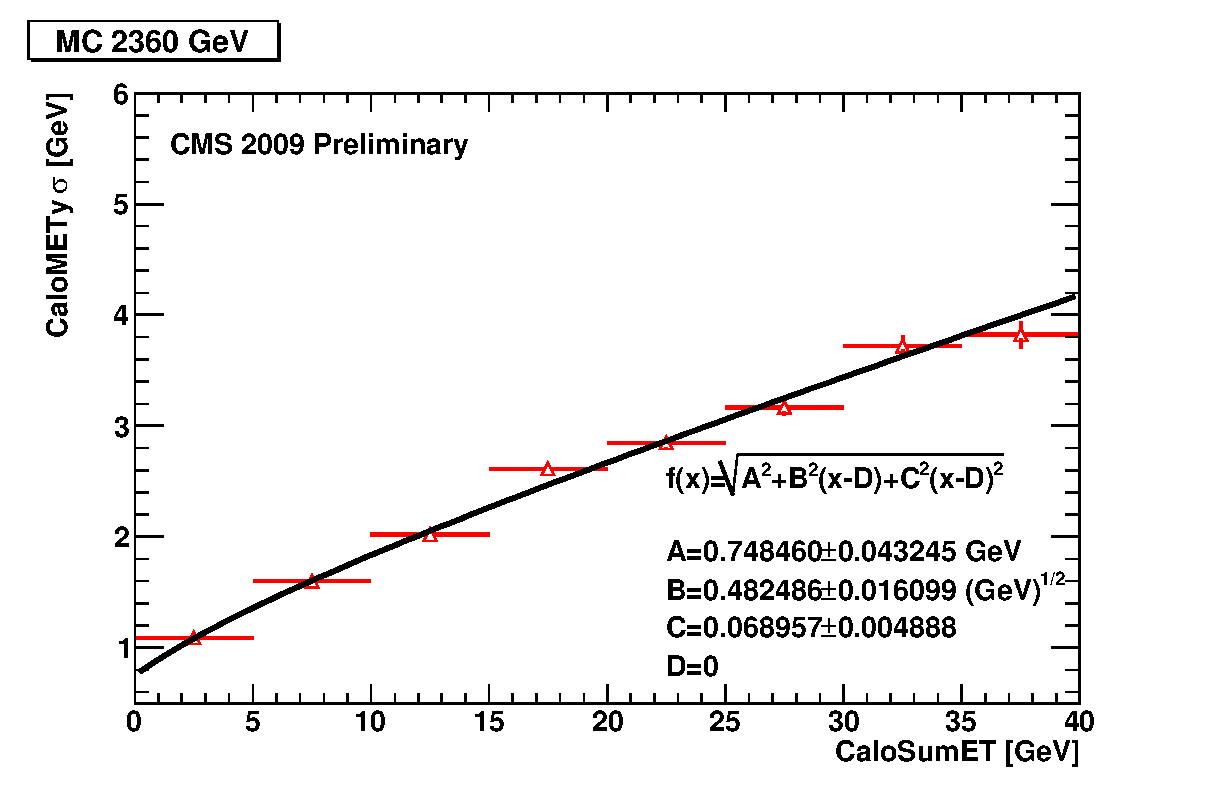
\includegraphics[width=0.5\textwidth]{plots_DataVsMC_MB_2360GeV/final_metysigma_sumet_MC_2360.eps} \\
 \end{tabular}
 \caption{\small Fit of the $\sigma\left(\eymiss\right)$ vs. $\sum E_\text{T}$ for data and Monte Carlo at $2360$ GeV.\label{fig:MEySigma_vs_SumET_2360_fit}}
\end{figure}

\clearpage

\subsection[$\etmiss$ and $\sumet$ dependence on $\eta$]{$\etmissB$ and $\sumetB$ dependence on $\boldsymbol{\eta}$} \label{sec:MetVarVsIeta_2360}

Here we present the same analysis as the one presented in Section~\ref{sec:MetVarVsIeta_900}, repeated for the $2360$~GeV data. 

\begin{figure}[h!]
 \centering
 \begin{tabular}{ll}
  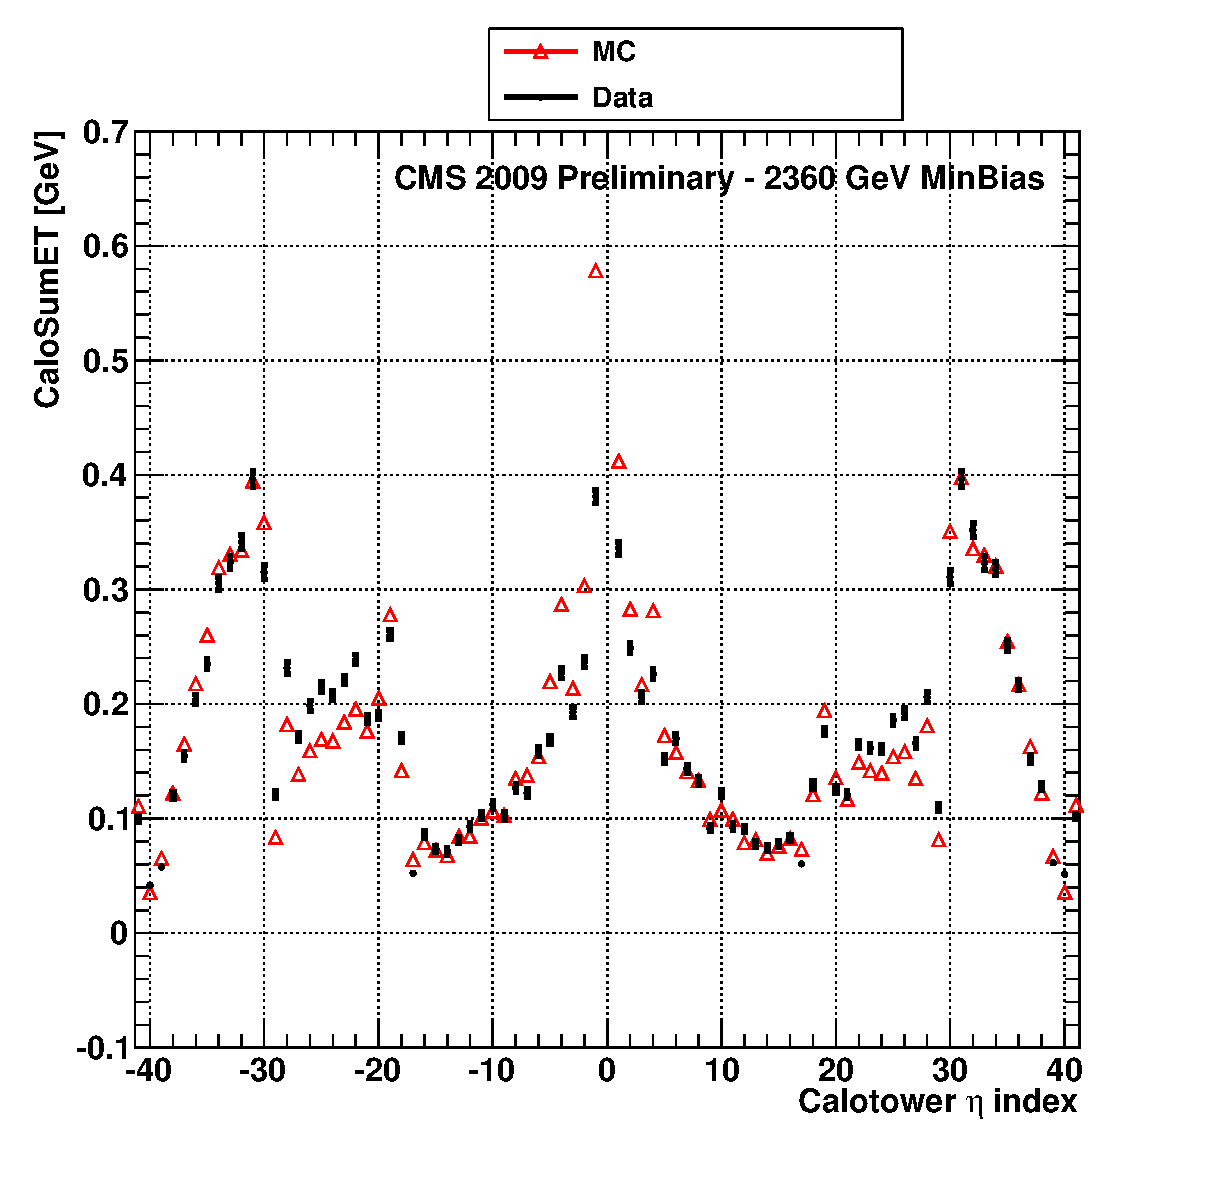
\includegraphics[width=0.5\textwidth]{plots_DataVsMC_MB_2360GeV/g_caloSumetMean_vs_ieta_2360.eps} &
  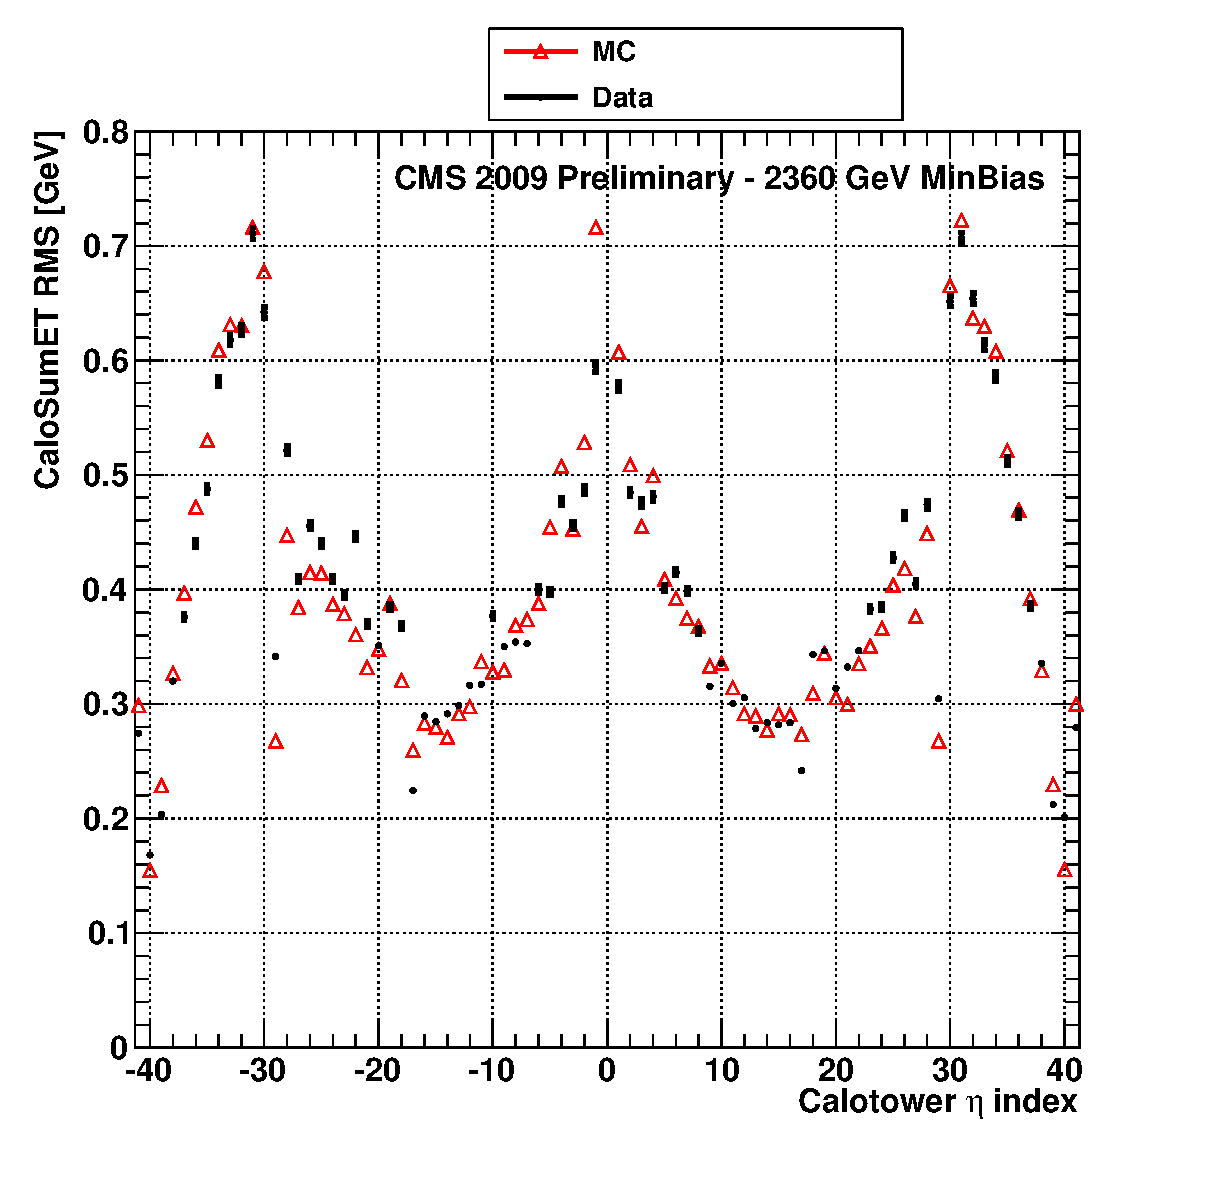
\includegraphics[width=0.5\textwidth]{plots_DataVsMC_MB_2360GeV/g_caloSumetRMS_vs_ieta_2360.eps} \\
 \end{tabular}
 \caption{\small Comparison of the $\sumet$ Mean vs. $i\eta$ of calotowers and $\sumet$ RMS vs. $i\eta$ of calotowers between 
          data and Monte Carlo at $2360$ GeV.\label{fig:SumET_MeanRMS_vs_ieta_2360}}
\end{figure}

\begin{figure}[h!]
 \centering
 \begin{tabular}{ll}
  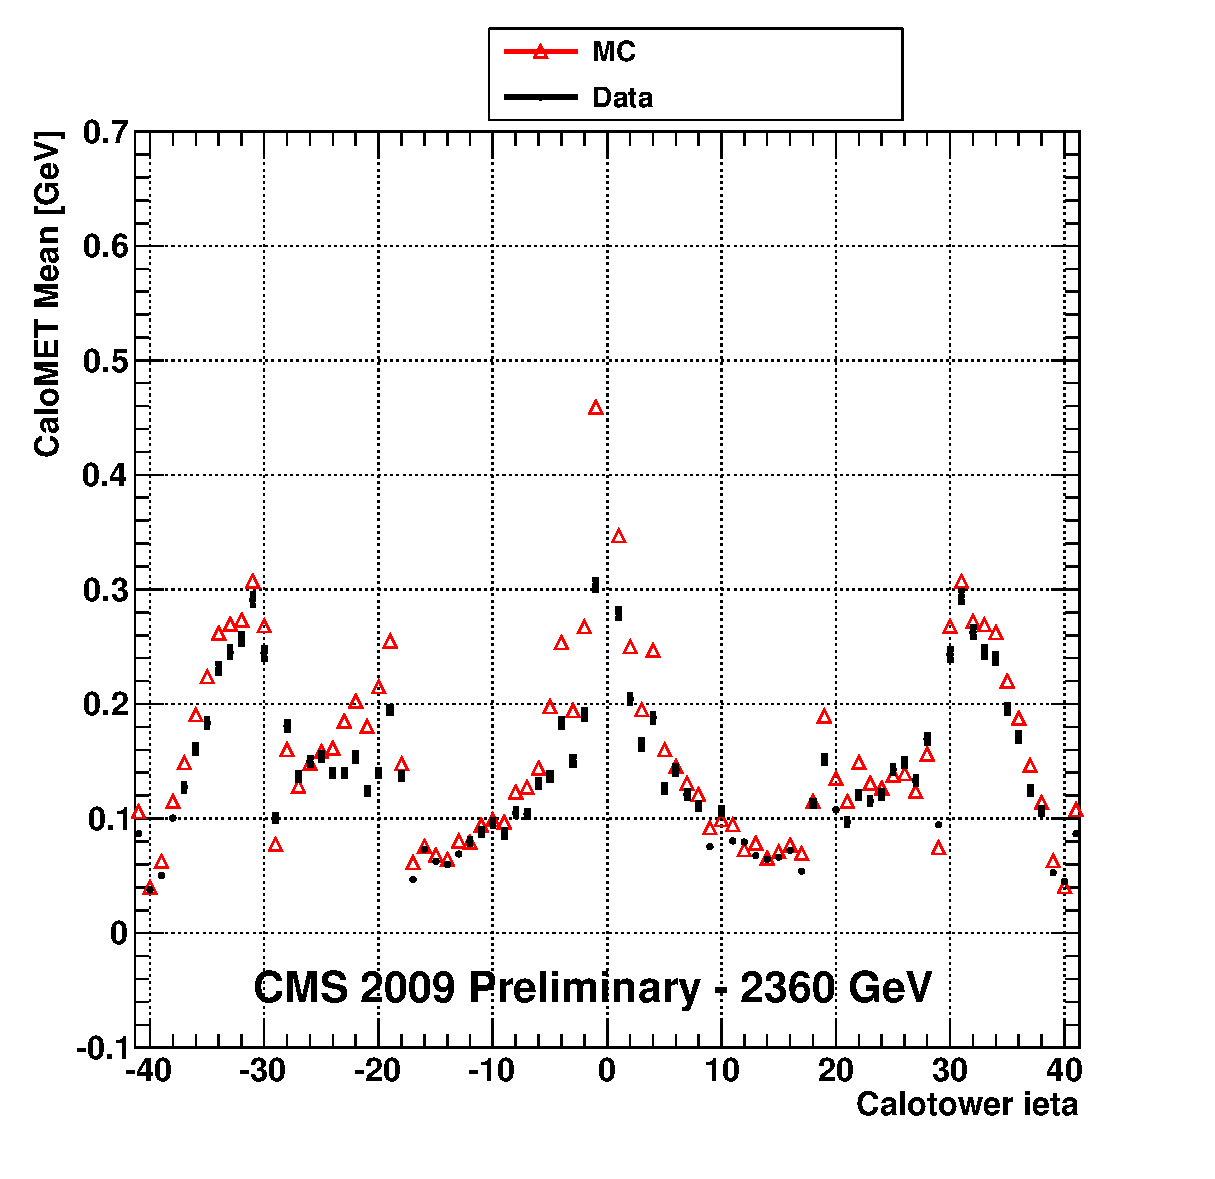
\includegraphics[width=0.5\textwidth]{plots_DataVsMC_MB_2360GeV/g_calometPtMean_vs_ieta_2360.eps} &
  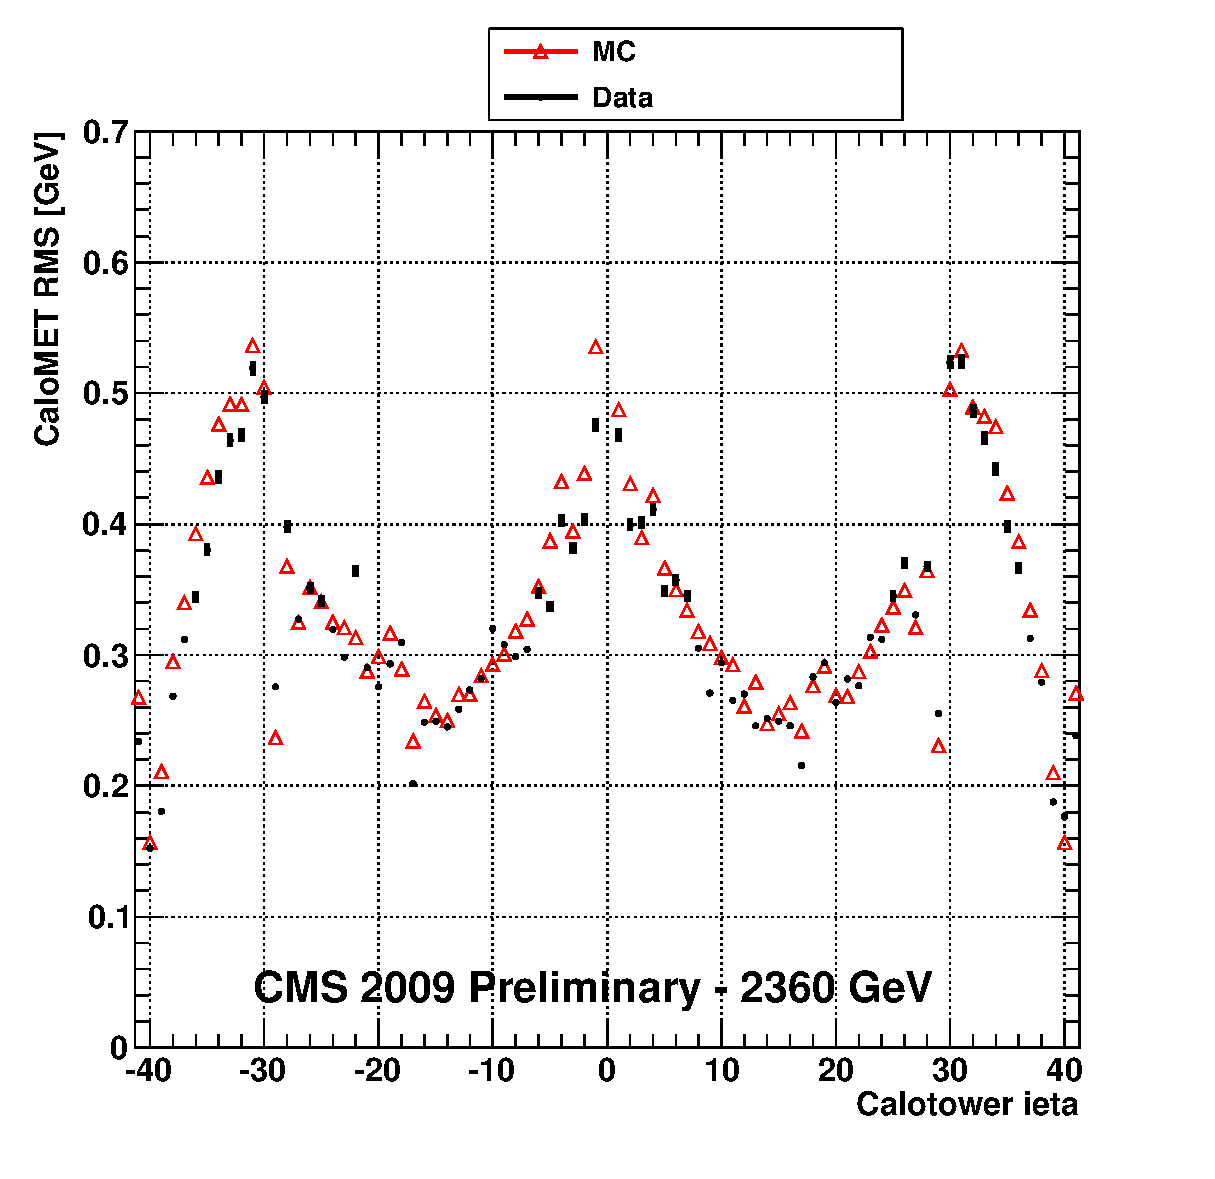
\includegraphics[width=0.5\textwidth]{plots_DataVsMC_MB_2360GeV/g_calometPtRMS_vs_ieta_2360.eps} \\
 \end{tabular}
 \caption{\small Comparison of the $\etmiss$ Mean vs. $i\eta$ of calotowers and $\etmiss$ RMS vs. $i\eta$ of calotowers between 
          data and Monte Carlo at $2360$ GeV.\label{fig:MET_MeanRMS_vs_ieta_2360}}
\end{figure}

\begin{figure}[h!]
 \centering
 \begin{tabular}{ll}
  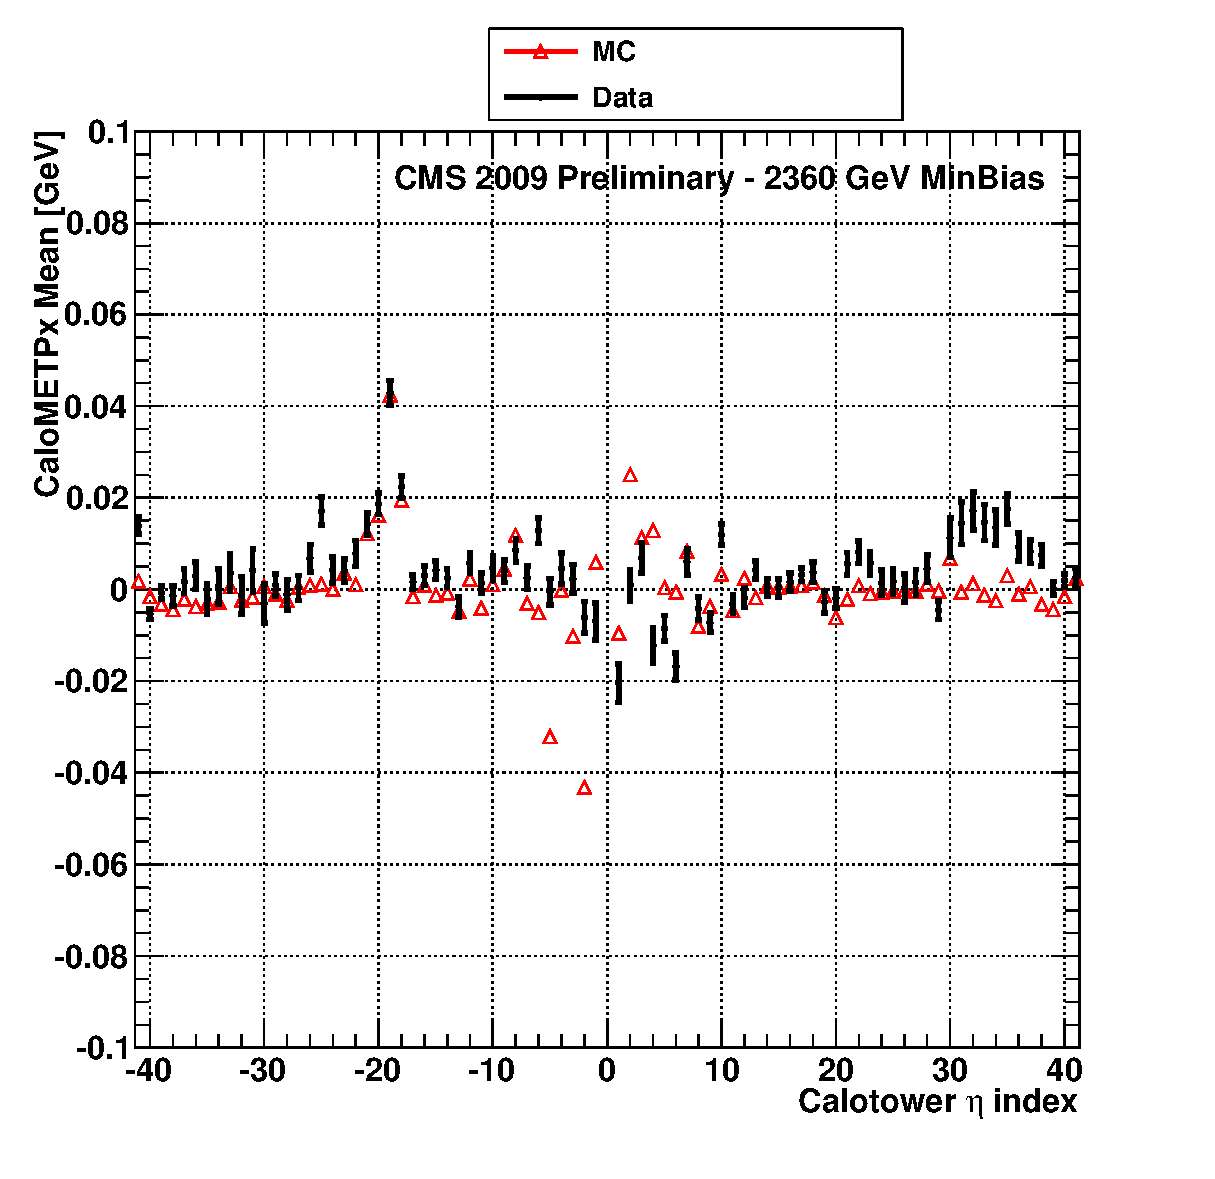
\includegraphics[width=0.5\textwidth]{plots_DataVsMC_MB_2360GeV/g_calometPxMean_vs_ieta_2360.eps} &
  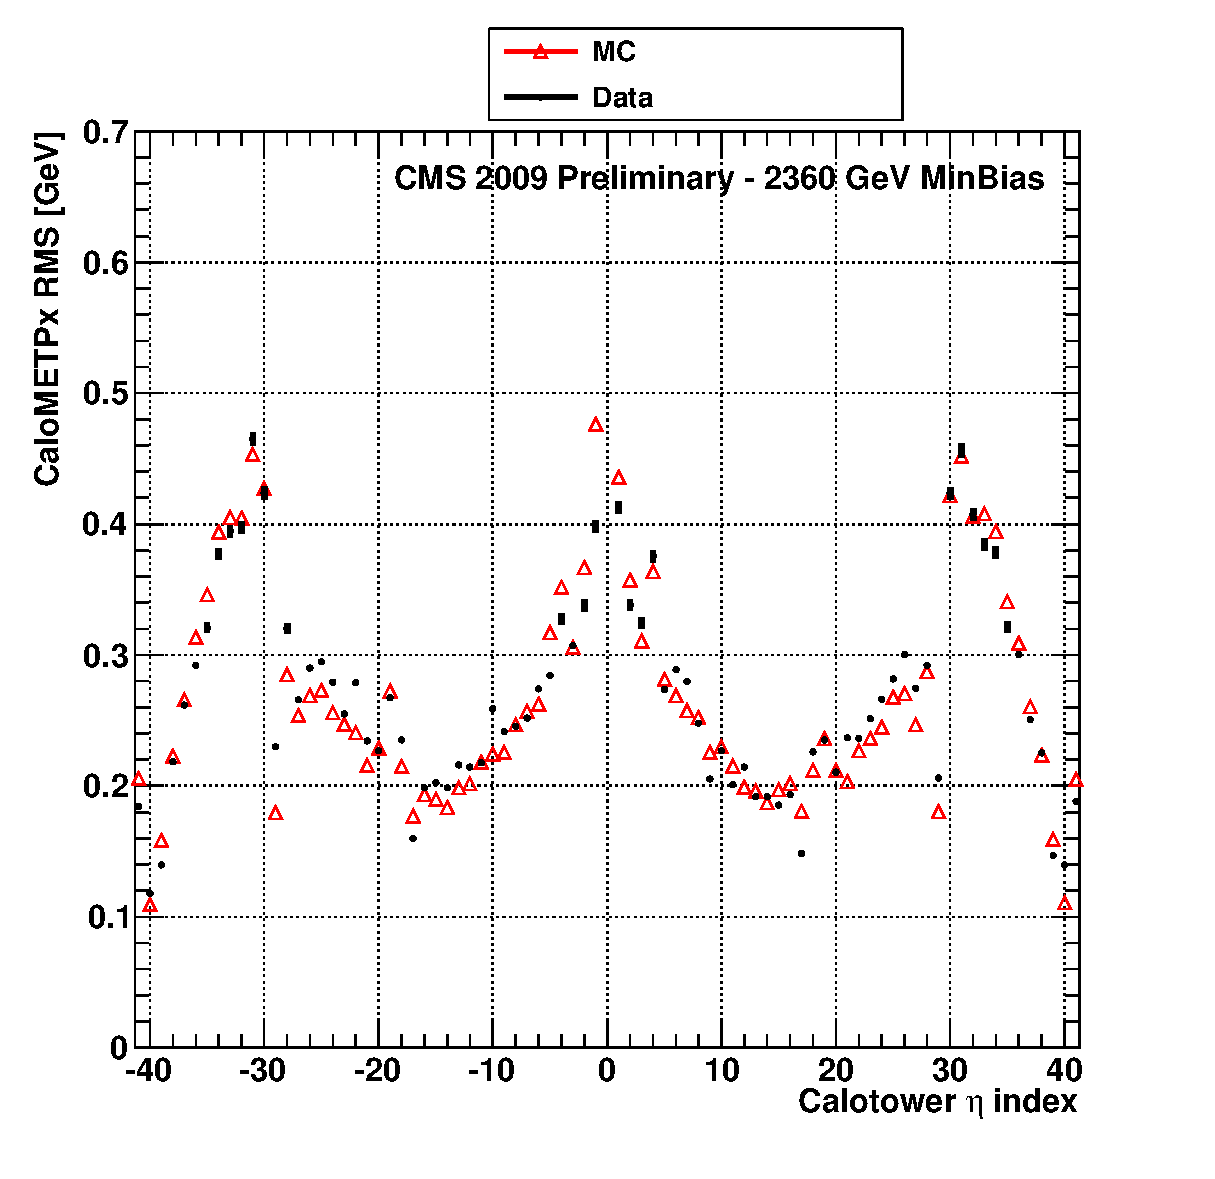
\includegraphics[width=0.5\textwidth]{plots_DataVsMC_MB_2360GeV/g_calometPxRMS_vs_ieta_2360.eps} \\
 \end{tabular}
 \caption{\small Comparison of the $\exmiss$ Mean vs. $i\eta$ of calotowers and $\exmiss$ RMS vs. $i\eta$ of calotowers between 
          data and Monte Carlo at $2360$ GeV.\label{fig:METx_MeanRMS_vs_ieta_2360}}
\end{figure}

\begin{figure}[h!]
 \centering
 \begin{tabular}{ll}
  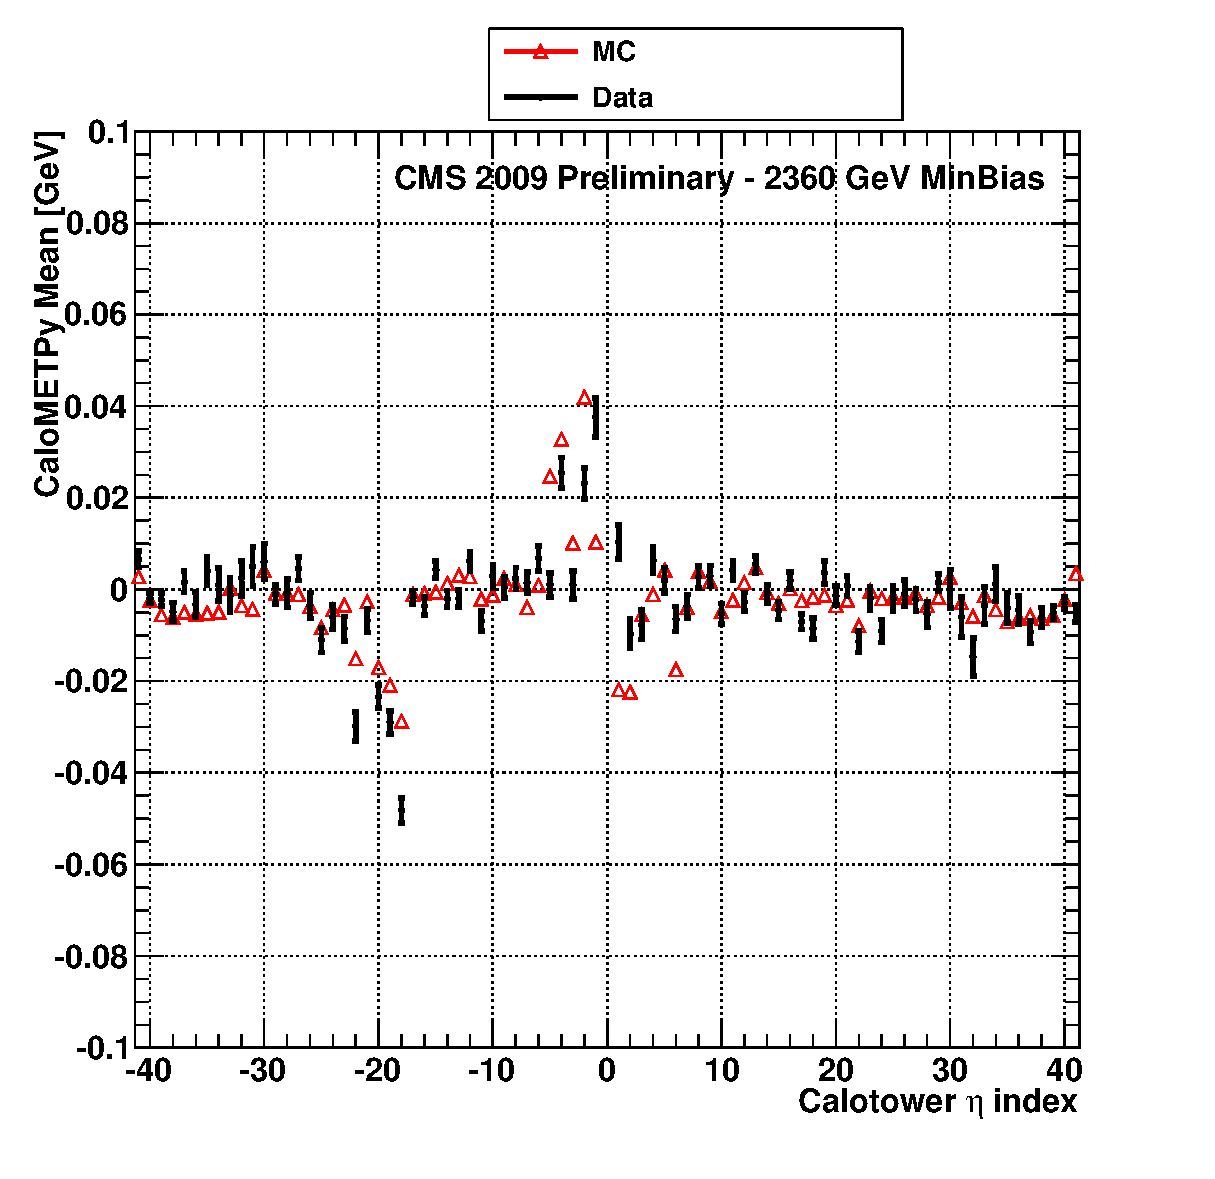
\includegraphics[width=0.5\textwidth]{plots_DataVsMC_MB_2360GeV/g_calometPyMean_vs_ieta_2360.eps} &
  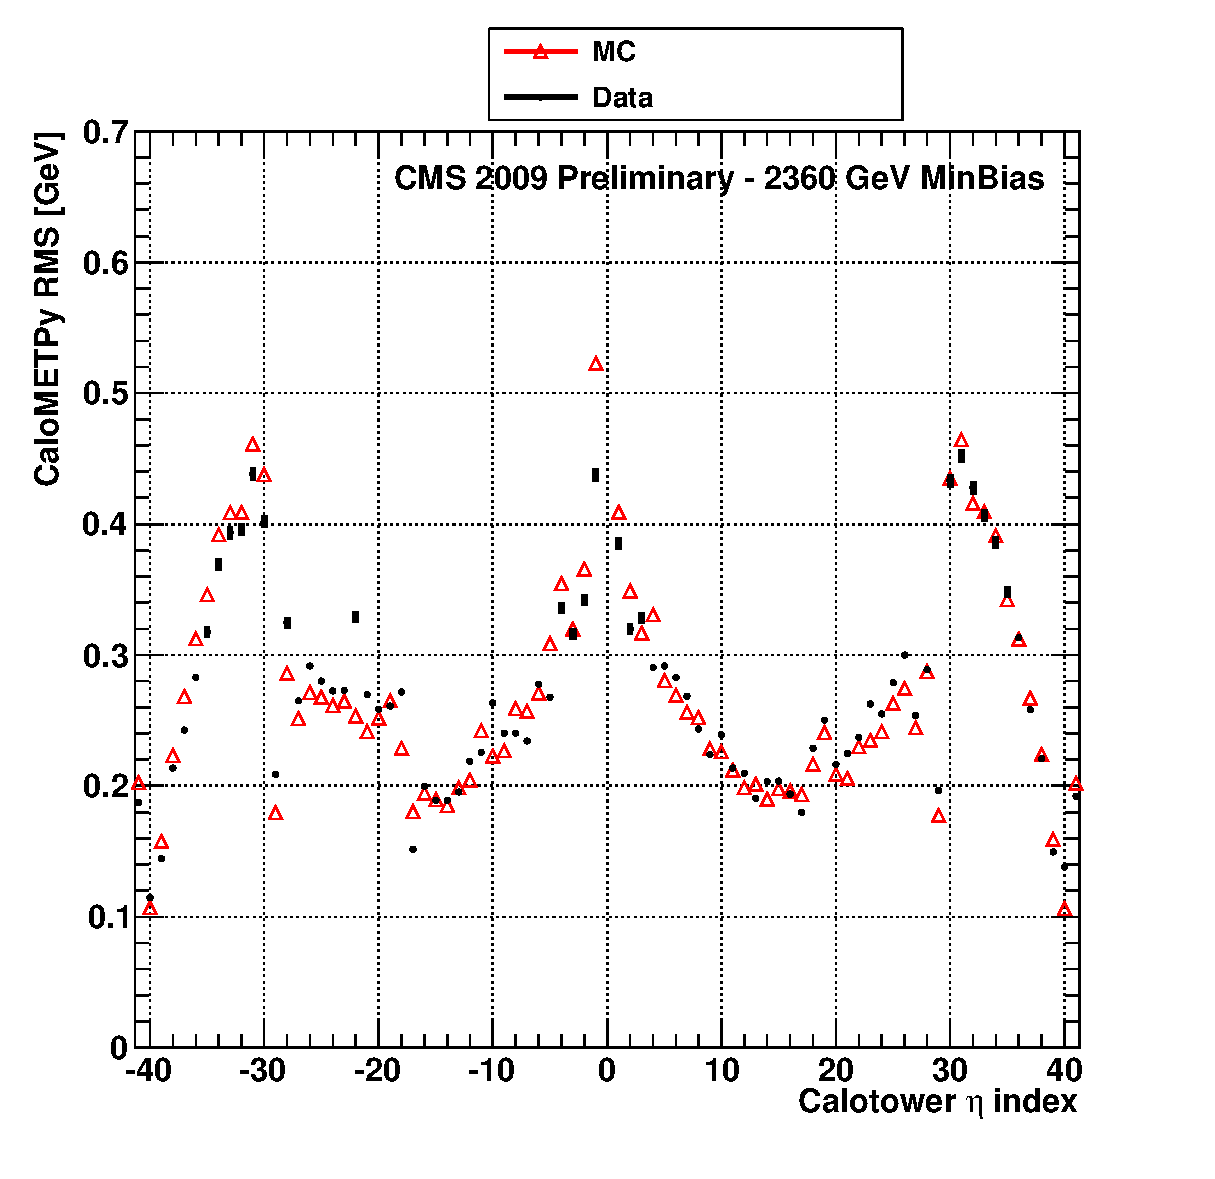
\includegraphics[width=0.5\textwidth]{plots_DataVsMC_MB_2360GeV/g_calometPyRMS_vs_ieta_2360.eps} \\
 \end{tabular}
 \caption{\small Comparison of the $\eymiss$ Mean vs. $i\eta$ of calotowers and $\eymiss$ RMS vs. $i\eta$ of calotowers between 
          data and Monte Carlo at $2360$ GeV.\label{fig:METy_MeanRMS_vs_ieta_2360}}
\end{figure}


\clearpage
